% ------------------------------------------------------------------------
% Modelo de Trabalho de Conclusão de Curso em conformidade com 
% ABNT NBR 14724:2011: Informacao e documentacao - Trabalhos academicos -
% Apresentacao
% ------------------------------------------------------------------------

\documentclass[12pt, oneside, a4paper, brazil]{abntex2}
  % ---
  % Pacotes básicos 
  % ---
  \usepackage{lmodern}			     % Usa a fonte Latin Modern			
  \usepackage[T1]{fontenc}		   % Selecao de codigos de fonte.
  \usepackage[utf8]{inputenc}		 % Codificacao do documento (conversão automática dos acentos)
  \usepackage{lastpage}			     % Usado pela Ficha catalográfica
  \usepackage{indentfirst}		   % Indenta o primeiro parágrafo de cada seção.
  \usepackage{color,xcolor}			 % Controle das cores
  \usepackage{graphicx}			     % Inclusão de gráficos
  \usepackage{microtype} 			   % para melhorias de justificação
  \usepackage[alf]{abntex2cite}	 % Citações padrão ABNT
  \usepackage{lipsum}            % Pode ser removido no final
  \usepackage{listingsutf8}
  
  \usepackage{hyperref}
  \usepackage{listings}
  \usepackage{xcolor}
  
  
  
  % Altera o nome padrão do rótulo usado no comando \autoref{}
  \renewcommand{\lstlistingname}{Código}
  % Altera o rótulo a ser usando no elemento pré-textual "Lista de código"
  \renewcommand{\lstlistlistingname}{Lista de códigos}
  
  % Configura a ``Lista de Códigos'' conforme as regras da ABNT (para abnTeX2)
  \begingroup\makeatletter
  \let\newcounter\@gobble\let\setcounter\@gobbletwo
    \globaldefs\@ne \let\c@loldepth\@ne
    \newlistof{listings}{lol}{\lstlistlistingname}
    \newlistentry{lstlisting}{lol}{0}
  \endgroup
  
  \renewcommand{\cftlstlistingaftersnum}{\hfill--\hfill}
  
  \let\oldlstlistoflistings\lstlistoflistings
  \renewcommand{\lstlistoflistings}{%
     \begingroup%
     \let\oldnumberline\numberline%
     \renewcommand{\numberline}{\lstlistingname\space\oldnumberline}%
     \oldlstlistoflistings%
     \endgroup}
  
  \definecolor{fundo}{HTML}{DCDCDC}
  
  \lstdefinestyle{estiloCodigos}{
      alsoother={0123456789_},
      backgroundcolor=\color{fundo},    % Cor de fundo
      basicstyle=\ABNTEXfontereduzida, 
      breakatwhitespace=false,          
      breaklines=true,                  
      captionpos=b,                     
      commentstyle=\color{green},       % cor de comentário
      deletekeywords={...},             % keywords excluídas da linguagem
      escapeinside={\%*}{*)},           % if you want to add LaTeX within your code
      extendedchars=true,               % lets you use non-ASCII characters; for 8-bits encodings only, does not work with UTF-8
      frame=single,                    % adds a frame around the code
      inputencoding=utf8,
      keepspaces=true,                 % keeps spaces in text, useful for keeping indentation of code (possibly needs columns=flexible)
      keywordstyle=\color{blue},       % keyword style
      literate={á}{{\'a}}1 {ã}{{\~a}}1 {é}{{\'e}}1 {è}{{\`{e}}}1 {ê}{{\^{e}}}1 {ë}{{\¨{e}}}1 {É}{{\'{E}}}1 {Ê}{{\^{E}}}1 {û}{{\^{u}}}1 {ú}{{\'{u}}}1 {â}{{\^{a}}}1 {à}{{\`{a}}}1 {á}{{\'{a}}}1 {ã}{{\~{a}}}1 {Á}{{\'{A}}}1 {Â}{{\^{A}}}1 {Ã}{{\~{A}}}1 {ç}{{\c{c}}}1 {Ç}{{\c{C}}}1 {õ}{{\~{o}}}1 {ó}{{\'{o}}}1 {ô}{{\^{o}}}1 {Õ}{{\~{O}}}1 {Ó}{{\'{O}}}1 {Ô}{{\^{O}}}1 {î}{{\^{i}}}1 {Î}{{\^{I}}}1 {í}{{\'{i}}}1 {Í}{{\~{Í}}}1,
      % if you want to add more keywords to the set
      morekeywords={*, :-},
      numberbychapter=false,
      numbers=left,                    % where to put the line-numbers; possible values are (none, left, right)
      numbersep=5pt,                   % how far the line-numbers are from the code
      % the style that is used for the line-numbers
      %numberstyle=\tiny\color{theframe}\sffamily, 
      numberstyle=\tiny\sffamily, 
      %rulecolor=\color{theframe},         % if not set, the frame-color may be changed on line-breaks within not-black text (e.g. comments (green here))
      showspaces=false,                % show spaces everywhere adding particular underscores; it overrides 'showstringspaces'
      showstringspaces=false,          % underline spaces within strings only
      showtabs=false,                  % show tabs within strings adding particular underscores
      stepnumber=1,                    % the step between two line-numbers. If it's 1, each line will be numbered
      %stringstyle=\color{mymauve}\itshape,     % string literal style
      stringstyle=\ttfamily,     % string literal style
      tabsize=2,                       % sets default tabsize to 2 spaces
      title=\lstname,                  % show the filename of files included with \lstinputlisting; also try caption instead of title
      framexleftmargin=10pt,
      framexleftmargin=15pt
  }
  
  \lstdefinelanguage{JavaScript}{
    keywords={typeof, new, true, false, catch, function, return, null, catch, switch, var, if, in, while, do, else, case, break},
    keywordstyle=\color{blue}\bfseries,
    ndkeywords={class, export, boolean, throw, implements, import, this},
    ndkeywordstyle=\color{darkgray}\bfseries,
    identifierstyle=\color{black},
    sensitive=false,
    comment=[l]{//},
    morecomment=[s]{/*}{*/},
    commentstyle=\color{purple}\ttfamily,
    stringstyle=\color{red}\ttfamily,
    morestring=[b]',
    morestring=[b]"
  }
  
  
  \lstset{escapechar=@,style=estiloCodigos}
  
  
  \titulo{Desempenho na comunicação \\ entre serviços Web}
\autor{Marlon Diego Casagranda França}
\local{Araquari -- SC}
\data{Novembro de 2017}
\orientador{Prof. Dr. Eduardo da Silva}
  % Informações de dados para CAPA e FOLHA DE ROSTO
  \instituicao{%
    Instituto Federal Catarinense -- IFC
    \par
    Câmpus Araquari
    \par
    Bacharelado em Sistemas de Informação}
  \tipotrabalho{Monografia (Graduação)}
  % O preambulo deve conter o tipo do trabalho, o objetivo, 
  % o nome da instituição e a área de concentração 
  \preambulo{Trabalho de conclusão de curso apresentado como requisito parcial para a obtenção do grau de bacharel em Sistemas de Informação do Instituto Federal Catarinense.}
  
  
  % Configurações de aparência do PDF final
  % informações do PDF
  \makeatletter
  \hypersetup{
       %pagebackref=true,
      pdftitle={\@title}, 
      pdfauthor={\@author},
       pdfsubject={\imprimirpreambulo},
      pdfcreator={LaTeX with abnTeX2},
      pdfkeywords={abnt}{latex}{abntex}{abntex2}{trabalho acadêmico}, 
      colorlinks=true,       		% false: boxed links; true: colored links
       linkcolor=blue,          	% color of internal links
       citecolor=blue,        		% color of links to bibliography
       filecolor=magenta,     		% color of file links
      urlcolor=blue,
      bookmarksdepth=4
  }
  \makeatother
  
  % Espaçamentos entre linhas e parágrafos 
  
  \setlength{\parindent}{1.3cm}			% O tamanho do parágrafo é dado por:
  \setlength{\parskip}{0.2cm}  			% Controle do espaçamento entre um parágrafo e outro:
  
  
  % Início do documento
  \begin{document}
  %\selectlanguage{english}
  \selectlanguage{brazil} 				% Seleciona o idioma do documento (conforme pacotes do babel)
  \frenchspacing 							    % Retira espaço extra obsoleto entre as frases.
  
  % ELEMENTOS PRÉ-TEXTUAIS
  \imprimircapa % Capa
  \imprimirfolhaderosto*		% Folha de rosto
                            % (o * indica que haverá a ficha bibliográfica)
  
  % Inserir a ficha bibliografica
  
  % Isto é um exemplo de Ficha Catalográfica, ou ``Dados internacionais de 
  % catalogação-na-publicação''. Utilizar este modelo como referência. 
  % Porém, provavelmente a biblioteca fornecerá um PDF com a ficha catalográfica 
  % definitiva após a defesa do trabalho. Quando estiver com o documento, salve-o como PDF 
  % no diretório do seu projeto e substitua todo o conteúdo de implementação deste arquivo 
  % pelo comando abaixo:
  %
  % \begin{fichacatalografica}
  %     \includepdf{fig_ficha_catalografica.pdf}
  % \end{fichacatalografica}
  
  \begin{fichacatalografica}
	\sffamily
	\vspace*{\fill}					% Posição vertical
	\begin{center}					% Minipage Centralizado
	\fbox{\begin{minipage}[c][8cm]{13.5cm}		% Largura
	\small
	\imprimirautor
	%Sobrenome, Nome do autor
	
	\hspace{0.5cm} \imprimirtitulo  / \imprimirautor. --
	\imprimirlocal, \imprimirdata-
	
	\hspace{0.5cm} \pageref{LastPage} p. : il. (algumas color.) ; 30 cm.\\
	
	\hspace{0.5cm} \imprimirorientadorRotulo~\imprimirorientador\\
	
	\hspace{0.5cm}
	\parbox[t]{\textwidth}{\imprimirtipotrabalho~--~\imprimirinstituicao,
	\imprimirdata.}\\
	
	\hspace{0.5cm}
		1. Comunicação.
		2. REST.
		2. GraphQL.
		3. Desempenho.
		I. Orientador.
		II. Instituto Federal Catarinense.
		III. Câmpus Araquari.
		IV. Título 			
	\end{minipage}}
	\end{center}
\end{fichacatalografica}
% ---

  
  
  % Inserir folha de aprovação
  
  % Exemplo de Folha de aprovação, elemento obrigatório da NBR 14724/2011 (seção 4.2.1.3). 
  % Utilizar este modelo até a aprovação do trabalho. Após isso, substitua todo o conteúdo 
  % deste arquivo por uma imagem da página assinada pela banca com o comando abaixo:
  %
  % \includepdf{folhadeaprovacao_final.pdf}
  %
  \begin{folhadeaprovacao}
  
    \begin{center}
      {\ABNTEXchapterfont\large\imprimirautor}
  
      \vspace*{\fill}\vspace*{\fill}
      \begin{center}
        \ABNTEXchapterfont\bfseries\Large\imprimirtitulo
      \end{center}
      \vspace*{\fill}
      
      \hspace{.45\textwidth}
      \begin{minipage}{.5\textwidth}
          \imprimirpreambulo
      \end{minipage}%
      \vspace*{\fill}
     \end{center}
          
     Trabalho aprovado. \imprimirlocal, 24 de novembro de 2016:
  
     \assinatura{\textbf{\imprimirorientador} \\ Orientador} 
     \assinatura{\textbf{Prof. Rafael de Moura Speroni} \\ Convidado 1}
     \assinatura{\textbf{Diego Contezini} \\ Convidado 2}
     %\assinatura{\textbf{Professor} \\ Convidado 3}
     %\assinatura{\textbf{Professor} \\ Convidado 4}
        
     \begin{center}
      \vspace*{0.5cm}
      {\large\imprimirlocal}
      \par
      {\large\imprimirdata}
      \vspace*{1cm}
    \end{center}
    
  \end{folhadeaprovacao}
  % ---
  
  % % Dedicatória
\begin{dedicatoria}
   \vspace*{\fill}
   \centering
   \noindent
   \textit{ Dedicatória do trabalho de conclusão que deve \\
   ser algo breve e conciso.} \vspace*{\fill}
\end{dedicatoria}


% Agradecimentos
\begin{agradecimentos}
Página com os agradecimentos do autor à pessoas importantes para a realização do trabalho.
\end{agradecimentos}

% Epígrafe
\begin{epigrafe}
    \vspace*{\fill}
	\begin{flushright}
		\textit{``Colocar alguma frase importante que, \\
		tenha motivado o autor no decorrer do desenvolvimento \\
		do trabalho.'' \\
		(Referência de local da frase)}
	\end{flushright}
\end{epigrafe}

  % RESUMOS
% resumo em português
\setlength{\absparsep}{18pt} % ajusta o espaçamento dos parágrafos do resumo
\begin{resumo}

    Com a ascensão de dispositivos móveis que reivindicam uma parcela cada vez maior do tráfego de internet, otimizar o desempenho da busca de dados torna-se mais importante. A arquitetura REST tem sido durante muito tempo a solução mais comum ao desenvolver APIs Web, mas o GraphQL tem se tornado, em tempos recentes, uma alternativa interessante ao REST. 
    
    O presente trabalho aborda as principais técnicas e conhecimentos sobre comunicação entre aplicações Web. Também é realizado neste trabalho um experimento, tendo como principal parâmetro de comparação o desempenho de APIs implementando REST e GraphQL quando realizados buscas de objetos aninhamos. Protótipos de cada API foram implementados e usados para realizar medições do desempenho de cada técnica. O GraphQL apresentou um melhor desempenho em praticamente todos os cenários executados no experimento.

\textbf{Palavras-chave}: Comunicação. REST. GraphQL. Desempenho.

\end{resumo}

% resumo em inglês
\begin{resumo}[Abstract]
 
   This is the english abstract.

   \vspace{\onelineskip}
 
   \noindent 
   \textbf{Keywords}: latex. abntex. text editoration.
 
\end{resumo}

  % ---
% inserir lista de ilustrações
% ---
\pdfbookmark[0]{\listfigurename}{lof}
\listoffigures*
\cleardoublepage
% ---

% ---
% inserir lista de tabelas
% ---
\pdfbookmark[0]{\listtablename}{lot}
\listoftables*
\cleardoublepage
% ---
% inserir lista de codigos
% ---
\pdfbookmark[0]{\lstlistlistingname}{lol}
\begin{KeepFromToc}
\lstlistoflistings
\end{KeepFromToc}
\cleardoublepage
% ---

% ---
% inserir lista de abreviaturas e siglas
% ---
\begin{siglas}
  \item[IoT] Internet of Things
  \item[API] Application Program Interface
  \item[SOAP] Simple Object Access Protocol
  \item[REST] Representational State Transfer
  \item[HTTP] Hypertext Transfer Protocol
  \item[HTTPS] Hypertext Transfer Protocol Secure
  \item[URL] Uniform Resource Locator
  \item[IPC] Interprocess Communications
  \item[CPU] Central Processing Unit
  \item[SOA] Service Oriented Architecture
  \item[TI] Tecnologia da Informação
  \item[W3C] World Wide Web Consortium  
  \item[XML] Extensible Markup Language
  \item[JSON] JavaScript Object Notation
  \item[RPC] Remote Procedure Call
  \item[SMTP] Simple Mail Transfer Protocol
  \item[FTP] File Transfer Protocol
  \item[HATEOAS] Hypermedia as the Engine of Application State
  \item[WMS] Warehouse Management System
  \item[ERP] Enterprise Resource Planning
  \item[UUID] Universally unique identifier
  

\end{siglas}
% ---

% ---
% inserir lista de símbolos
% ---
\begin{simbolos}
  \item[$ \Delta $] Letra grega Delta
\end{simbolos}
% ---

% ---
% inserir o sumario
% ---
\pdfbookmark[0]{\contentsname}{toc}
\tableofcontents*
\cleardoublepage
% ---
  
  % ----------------------------------------------------------
  % ELEMENTOS TEXTUAIS
  % ----------------------------------------------------------
  \textual
  
  % ---
  % Inclusão de capítulo de Introdução ao trabalho
  % ---
  % ----------------------------------------------------------
% Introdução (exemplo de capítulo sem numeração, mas presente no Sumário)
% ----------------------------------------------------------
\chapter[Introdução]{Introdução}
%\addcontentsline{toc}{chapter}{Introdução}
% ----------------------------------------------------------

Em um mundo cada vez mais interconectado, usuários constantemente exigem maior disponibilidade de informações através da Web. Essas informações não devem apenas estar acessíveis, como também é crucial que seja rápido o tempo para acessá-las. Com a expansão da Internet para dispositivos dos mais diversos tipos, tais como \textit{smartphones}, \textit{tablets} e dispositivos de IoT, questões como tempo de carregamento e consumo de banda vem se tornando fatores cada mais mais debatidos.

O uso de dispositivos móveis para acessar a Internet cresceu 63\% somente em 2016, como aponta o relatório de Previsão Global de Tráfego de Dados Móveis, elaborado pela Cisco. O tráfego de dados móveis passou de  4,4 exabytes \footnote{Um exabyte é equivalente a um bilhão de gigabytes e mil petabytes.} por mês em 2015, para uma média mensal de 7,2 exabytes em 2016. Esse aumento foi resultado de uma adição de cerca 429 milhões de novos dispositivos móveis à rede, sendo os \textit{smartphones} responsáveis pela maior parte deste crescimento \cite{cisco-network-report}.

Conforme \citeonline{load-time-effects}, usuários tendem a dar mais importância à velocidade em que recebem a informação do que a estética que ela é apresentada. O tempo de carregamento é um fator decisivo para a permanência em uma página Web, uma vez que a maioria dos usuários estão dispostos a aguardar de 6 a 10 segundos antes de abandonar qualquer página. Cada segundo de atraso pode resultar em uma redução de até 7\% nas taxas de conversão, o que para um \textit{e-commerce} que fatura mensalmente R\$ 100.000,00 por exemplo, pode potencialmente custar R\$ 84.000,00 em vendas não efetuadas em um ano.

Para atender estas novas demandas, nos últimos anos houve uma mudança para um modelo de computação chamado cliente/servidor, que aborda as falhas da computação centralizada. Claramente, o modelo de computação centralizado permanece válido em certos ambientes de negócios, no entanto, apesar de muitos benefícios, a computação centralizada é reconhecida como tendo promovido uma cultura de gerenciamento de informações que não conseguiu atender as necessidades de seus clientes.

Em 2010, ocorreu um grande avanço no número de APIs públicas impulsionado pela transição no modelo de comunicação entre aplicações distribuídas, em que estas passaram a utilizar amplamente o protocolo HTTP e o modelo cliente/servidor para a troca de informações através da Web \cite{tcc-ufsc}. A adoção do REST (REpresentational State Transfer) como o método predominante para construir APIs públicas tem ofuscado qualquer outra tecnologia ou abordagem nos últimos anos. Embora várias alternativas (principalmente SOAP) ainda estejam presentes no mercado, adeptos do modelo SOA para construção de aplicações tomaram uma posição definitiva contra eles e optaram por REST como modelo de comunicação e JSON como seu formato de mensagem \cite{programmableweb-rest-losing}.

Segundo \citeonline{rest-webservice}, REST é cada vez mais usado como alternativa ao “já antigo” SOAP em que a principal crítica é a burocracia, algo que o REST possui em uma escala muito menor. REST é baseado no \textit{design} do protocolo HTTP, que já possui diversos mecanismos embutidos para representar recursos como código de \textit{status}, representação de tipos de conteúdo, cabeçalhos, etc. O principal nesta arquitetura são as URLs do sistema e os \textit{resources} \footnote{resource é um recurso, entidade}, aproveitando os métodos HTTP para se comunicar.

Entretanto, com o aumento do uso do REST como modelo de comunicação das APIs, algumas limitações foram expostas, prejudicando o desempenho destas APIs em aspectos cruciais. Clientes com rotinas complexas necessitam realizar consultas complexas, buscando objetos aninhados com diversos relacionamentos. Como uma API REST expõe exclusivamente recursos, é necessário executar diversas buscas no servidor para que algumas rotinas possam ser processadas pelo cliente, uma vez que nem todas as informações necessárias estão presentes na resposta de uma única consulta.

Além disso, em tais cenários são necessárias diversas chamadas na API, pois uma só consulta pode não conter toda informação necessária. Ainda, grande parte destas chamadas irão retornar dados desnecessários ao contexto da rotina que a executou. Esta prática é conhecida como \textit{over-fetching} e ocorre pois é responsabilidade do servidor da API montar o conteúdo da resposta, resultando no tráfego de dados desnecessários.

Foram propostas múltiplas soluções para aumentar a eficiência na busca de dados, algumas em relação aos formatos de consulta e resposta das requisições, enquanto outras estão otimizando o número de solicitações na rede. Uma tendência recente envolve um modelo de consultas declarativas de dados, em que as aplicações clientes especificam quais dados precisam, em vez de buscar tudo a partir de um local específico definido por um URL. Desta forma, estes modelos otimizaram a comunicação com os servidores para obter os dados de forma eficiente: esta é a proposta do GraphQL.

Construído pelos desenvolvedores do Facebook para atender as necessidades internas da rede social em 2012, o GraphQL foi lançado ao público em geral em 2015, e já vem ganhando diversos adeptos. Com a promessa de mitigar alguns problemas crônicos do \textit{design} do REST, como versionamento de APIs, múltiplas viagens de ida e volta e excesso de dados trafegados na rede, a abordagem do Facebook já vem sendo usada por diversas empresas.

REST é de fato, o modelo mais utilizado para comunicação entre cliente e servidor nas aplicações atuais. Este trabalho foca em identificar as diferenças em termos de tempo de carregamento, quantidade de dados trafegados e consumo de recursos entre aplicações REST e o ainda pouco conhecido GraphQL. Para isso, serão criados dois protótipos de API, um implementando o \textit{design} do REST e outro utilizando GraphQL como mecanismo para responder às consultas. O desempenho das duas APIs será então medido, com base em métricas quantitativas e será apresentado a análise dos resultados obtidos.

O restante deste trabalho está organizado da seguinte forma: o capítulo 2 apresenta a evolução das arquiteturas para construção de aplicações; o capítulo 3 aborda os modelos de comunicação entre aplicações, com informações sobre a evolução destes modelos e conceitos em geral, com ênfase nas duas tecnologias analisadas; o capítulo 4 apresenta o ambiente utilizado, as hipóteses levantadas, e detalhes das ferramentas e métricas utilizadas para a análise dos resultados; o capítulo 4 se resume na apresentação e análise dos resultados obtidos. Por fim, e não menos importante, será apresentada a conclusão.
  % ---
  % Inclusão de outros capitulos
  % ----------------------------------------------------------
% Histórico dos tipos de aplicações
% ----------------------------------------------------------
\chapter[Fundamentos]{Fundamentos}
%\addcontentsline{toc}{chapter}{Histórico}
% ----------------------------------------------------------


\section{IPC - Interprocess Communication}\label{sec:ipc}

Nem sempre um programa sequencial é a melhor solução para um determinado problema. Muitas vezes, as implementações são estruturadas na forma de várias tarefas inter-dependentes que cooperam entre si para atingir os objetivos da aplicação \cite{sistemas-op-mazierro}.

Diversos sistemas operacionais fornecem mecanismos para viabilizar a comunicação e o compartilhamento de dados entre aplicações. Coletivamente, as atividades habilitadas por estes mecanismos são chamadas de Interprocess Communications (IPC) \cite{microsoft-ipc}.

IPC consist em mecanismos que garantem a comunicação entre processos concorrentes e os acessos aos recursos compartilhados. Algumas formas de IPC facilitam a divisão de trabalho entre diversos processos especialistas, enquanto outras facilitam esta divisão entre computadores dentro de uma rede.

Normalmente, os aplicativos que fazer parte de uma comunicação através de IPC são categorizados como clientes ou servidores. Um cliente é um aplicativo ou um processo que solicita um serviço de alguma outra aplicação ou processo. Por outro lado um servidor é um aplicativo ou um processo que responde a uma solicitação de cliente. Muitas aplicações agem como um cliente e servidor, dependendo da situação \cite{microsoft-ipc}.

A figura \ref{fig:how-communication-works} mostra como ocorre a comunicação entre processos (P1 e P2). Esta troca de informação pode acontecer de duas maneiras: em duas etapas, ou de forma direta. A comunicação em duas etapas envolve um processo coordenador, que pode ser um interpretador em Python utilizado para dar início ao \textit{workflow} por exemplo. A comunicação direta é ilustrada na figura ligada por linhas pontilhadas e não necessita de intermediação de nenhum processo. Esta maneira de comunicação pode ser executada através de diversas formas, entre elas: \textit{Pipes}, \textit{Shared Memory}, \textit{Mapped Memory} e Arquivos compartilhados.

\begin{figure}
    \centering
    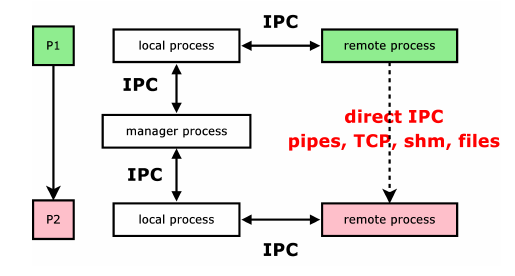
\includegraphics[width=0.7\textwidth]{figuras/ipc.png}
    \legend{Características dos mecanismos de comunicação \citeonline{sistemas-op-mazierro}}
    \label{fig:how-communication-works}
\end{figure}

\section{Cliente/Servidor}\label{sec:clientserver}

Também conhecido como arquitetura de duas camadas, o modelo cliente/servidor consiste em uma arquitetura em que a camada de apresentação se encontra no cliente e a camada de dados esta armazenada no servidor. Esta separação se opõe ao modelo centralizado amplamente utilizado até seu surgimento.

O processamento dos dados é dividido em duas partes distintas. Uma parte é a requerente de dados (cliente), e a outra parte é a provedora dos dados (servidor). O cliente envia durante sua execução uma ou mais solicitações ao servidor para realizar alguma tarefa específica. É dele a responsabilidade tanto de apresentar as informações para o usuário, quando executar as regras de negócio necessárias à aplicação. O servidor é responsável por armazenar os dados e prover um meio para que o cliente os consulte.

Desde a década de 1990, fornecedores de \textit{software} desenvolvem e trazem ao mercado muitas ferramentas para simplificar o desenvolvimento de aplicativos para a arquitetura cliente/servidor de 2 camadas. Algumas das mais conhecidas são: Microsoft Visual Basic, Delphi da Borland e PowerBuilder da Sybase. Estas ferramentas combinadas com milhões de desenvolvedores que sabem usá-las, significam que a abordagem de duas camadas cliente/servidor é uma solução econômica para certas classes de problemas.

Desde então, aplicações \textit{desktop} comunicando-se com o servidor de banco de dados se tornou um caso de uso normal. A maior parte da lógica de negócios foi incorporada dentro da aplicação \textit{desktop}. Portanto, esse estilo de clientes na aquitetura de duas camadas também foi chamado de \textit{fat clients}.

\begin{figure}[htbp]
    \centering
    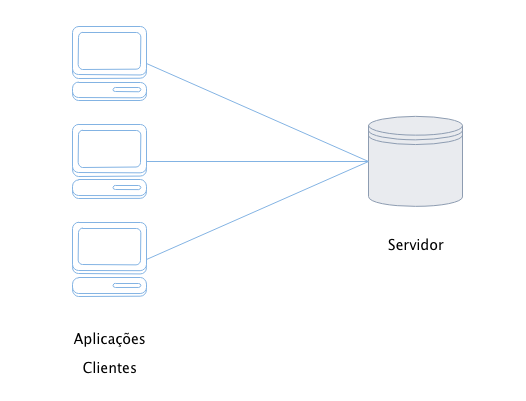
\includegraphics[width=0.7\textwidth]{figuras/client-server.png}
    \caption{Comunicação em duas camadas}
    \label{fig:two-tier}
\end{figure}

A figura \ref{fig:two-tier} ilustra como a arquitetura em duas camadas funciona, mantendo uma comunicação direta entre cliente e servidor, sem intermediarios entre as duas pontas. Visto que neste modelo as regras de negócio estão presentes na camada de aplicação, ele é frequentemente aplicado em ambientes homogêneos. A camada de banco de dados e a camada de aplicação estão fisicamente próximos, o que oferece um bom desempenho para as aplicações.

Por outro lado, o modelo cliente servidor em duas cadamas possui grandes desafios de escalabilidade. Quando múltiplos usúarios executam requisições simultaneas, a aplicação perde muito desempenho, dado ao fato que cada cliente precisa de conecções separadas e memória de CPU para processar as requisições. Entretando, um dos maiores problemas na arquitetura em duas camadas ocorre quando há mudanças na estrutura do banco de dados. A maioria das aplicações cliente dependem da estrutura do banco de dados impedindo qualquer remodelagem, criando um problema de estruturas legadas, e muitas vezes subutilizadas.

Esta modelo foi substituido pelo modelo de três camadas, muito mais eficiente, e que fornece uma maneira de dividir as funcionalidades envolvidas na manutenção e apresentação de uma aplicação.

\section{Aplicações Monolíticas}\label{sec:monolitico}

Conforme \citeonline{monolithic-definition} explica, uma aplicação monolítica é construída como uma única unidade de \textit{software}. Estas aplicações são construídas em três partes: um banco de dados (que consiste em tabelas geralmente em um sistema de gerenciamento de banco de dados), uma interface de usuário do lado do cliente (consistindo de páginas executando em um navegador ou aplicativos móveis) e um lado do servidor de aplicação. Esta aplicação do lado do servidor tratará as requisições HTTP, executará a regra de negócio, recuperará e atualizará dados do banco de dados e construirá as respostas para serem enviadas às aplicações clientes. Estas camadas representam uma aplicação monolítica - um único executável lógico. Para fazer alterações no sistema, é necessário criar e implantar uma versão atualizada do aplicativo do lado do servidor.

Uma aplicação monolítica é autônoma e independente de outras aplicações. A filosofia do projeto consiste em um aplicativo que não é responsável apenas por uma determinada tarefa, mas que também pode executar todos os passos necessários para completar uma determinada função, como é mostrado na figura \ref{fig:three-tier}.

\begin{figure}[htbp]
    \centering
    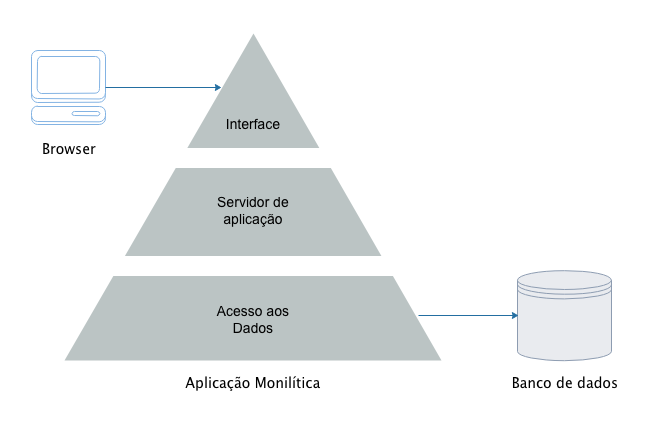
\includegraphics[width=0.7\textwidth]{figuras/monolithic-3-tier.png}
    \caption{Aplicação monolítica clássica em 3 camadas}
    \label{fig:three-tier}
\end{figure}

\citeonline{monolithic-extinction} afirma que as aplicações monolíticas são uma maneira natural para a evolução de uma aplicação. A maioria das aplicações começam com um único objetivo, ou um pequeno número de objetivos relacionados. Ao longo do tempo, novas funcionalidades são adicionados ao aplicativo para suportar as necessidades do negócio. Entretando, as aplicaçõies monolíticas apresentam algumas desvantagens, sendo alguns deles: 

\begin{itemize}
    \item Um único ponto de falha pode comprometer o funcionamento correto de todos os módulos do sistema.
    \item Baixa estalabilidade dado a necessidade de copiar toda a \textit{stack} para escalar horizontalmente.
    \item Base de código \textbf{gigante}, uma vez que toda a regra de negócio se encontra em uma só base.
    \item É necessário muita comunicação para que várias equipes de desenvolvedores trabalhem em paralelo. Esta sobrecarga diminui o ritmo de desenvolvimento.
\end{itemize}

Contudo, com a popularização dos \textit{frameworks} Javascript como Angular e Backbone, houve um movimento de desacoplamento da camada de visualização nas aplicações monolíticas. Foram criadas então as chamadas aplicações \textit{frontend}, responsáveis pela camada de apresentação, e sendo executadas em dispositivos móveis como \textit{smartphones} e \textit{tables} ou nos \textit{browsers desktop}. 

Esse movimento criou um modelo monolítico de duas camadas, ilustrado na figura \ref{fig:two-tier-monolithic}. A remoção da interdependência entre as camadas de interface e servidor de aplicação facilitou o escalonamento e a escalabilidade de cada uma das partes. Esta separação de conceitos foi o primeiro passo em direção a uma arquitetura orientada a serviços.

\begin{figure}[htbp]
    \centering
    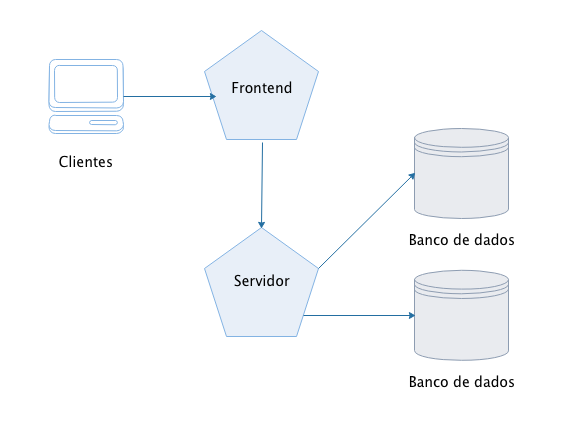
\includegraphics[width=0.7\textwidth]{figuras/monolithic-2-tier.png}
    \caption{Modelo monolítico de duas camadas}
    \label{fig:two-tier-monolithic}
\end{figure}

\section{SOA - Service Oriented Architecture}\label{sec:soa}

\citeonline{soa-cbdi} define SOA como políticas, práticas e frameworks que permitem que rotinas de aplicações sejam fornecidas e consumidas como conjuntos de serviços publicados em uma granularidade relevante para o consumidor do serviço. Os serviços podem ser invocados, publicados e descobertos e são abstraídos da implementação usando uma única forma de interface baseada em padrões.

Além de criar e expor serviços, \citeonline{soa-tech-target} assinala que o SOA tem a capacidade de aproveitar esses serviços de forma recursiva em aplicações (conhecidos como aplicativos compostos). O SOA vincula esses serviços à orquestração ou alavanca individualmente esses serviços. Desta forma, o SOA é visto como uma evolução das arquiteturas existentes, abordando a maioria dos principais sistemas como serviços e resgatando esses serviços em um único domínio onde eles formam soluções.

 O SOA permite a reutilização de ativos existentes, onde novos serviços podem ser criados a partir de uma infra-estrutura de sistemas de TI existente. Em outras palavras, ele permite que as empresas reutilizem aplicativos existentes e possibilita a interoperabilidade entre aplicações e tecnologias heterogêneas. Ele fornece um nível de flexibilidade que não era possível antes, no sentido de que:

\begin{itemize}
    \item Os serviços são componentes de software com interfaces bem definidas que são independentes da implementação. Um aspecto importante do SOA é a separação da interface de serviço (o que) da sua implementação (como). Esses serviços são consumidos por clientes que não estão preocupados com a forma como esses serviços irão executar suas solicitações;
    \item Os serviços são autônomos (executar tarefas predeterminadas) e vagamente acoplados (para independência);
    \item Serviços compostos podem ser construídos a partir de agregados de outros serviços;
\end{itemize}

Isso significa que o SOA é uma abordagem alinhada com o negócio, em que os aplicativos dependem dos serviços disponíveis para facilitar os processos de negócios. Um serviço é um componente de \textit{software} reutilizável e autônomo, fornecido por um provedor de serviços e consumido pelos solicitantes. O SOA cria uma visão de flexibilidade de TI que facilita a agilidade do negócio. Sua implementação envolve principalmente componentes de aplicativos corporativos e/ou em desenvolvimento que usam serviços, disponibilizando aplicativos como serviços para outras aplicações \cite{soa-book}.

\begin{figure}[htbp]
    \centering
    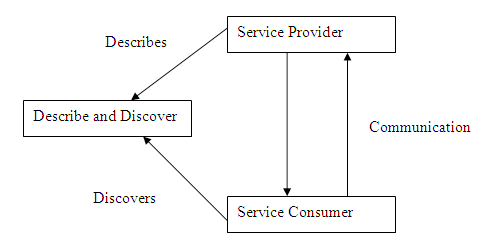
\includegraphics[width=0.7\textwidth]{figuras/soa.png}
    \caption{Service Oriented Architecture}
    \label{fig:soa}
\end{figure}

\citeonline{soa-intel} acrescenta que em um ambiente SOA típico, existe um provedor de serviços e um consumidor de serviços. Para que isso funcione, também é necessário um mecanismo para que eles possam se comunicar uns com os outros, como é ilustrado na figura \ref{fig:soa}. A W3C \footnote{World Wide Web Consortium} definiu um padrão aberto para que \textit{web services} possam implementar o SOA e habilitar a comunicação entre o provedor e o consumidor através de um protocolo baseado em XML: o \textit{Simple Object Access Protocol} (SOAP). Outros padrões também são usandos ou foram criados para realizar a comunicações entre os serviçoes SOA. Alguns basearam-se no \textit{design} do \textit{REpresentation State Transfer} (REST), utilizando tanto XML quando JSON para transportar os dados entre os serviços.

Em geral, há uma confusão entre o relacionamento entre SOA e \textit{web services}. \citeonline{soa-webservice} faz uma distinção entre o SOA e \textit{web services} do seguinte modo: \"Web services tratam-se de especificações de tecnologias, enquanto o SOA é um princípio de \textit{design} de \textit{software}. Notavelmente, Web services são um padrão de definição de interface adequado ao SOA e é neste ponto onde eles se conectam ao SOA". Portanto, o SOA é um padrão de arquitetura, enquanto os \textit{Web services} são serviços implementados usando um conjunto de padrões. Os \textit{Web services} são uma das maneiras em que é possível implementar o SOA. cujo os benefícios são que é possível alcançar uma abordagem neutra em relação a plataformas para acessar serviços e uma melhor interoperabilidade à medida que mais fornecedores suportam cada vez mais especificações.

  % ----------------------------------------------------------
% Protocolos de comunicaçào
% ----------------------------------------------------------
\chapter[Protocolos de Comunicação]{Protocolos de Comunicação}
%\addcontentsline{toc}{chapter}{Protocolos de Comunicação}
% ----------------------------------------------------------

Neste capítulo será apresentado alguns dos principais protocolos para a comunicação entre aplicações. Serão conduzidas breves abordagens dos protocolos RPC e SOAP, que hoje vem perdendo espaço no mercado, mas tiveram um papel muito importante para a evolução dos sistemas SOA. Em seguida, será mostrada uma descrição mais detalhada dos modelos de comunicação REST e GraphQL, uma vez que estes são os dois modelos a serem seguidos no estudo de caso.

Será apresentado as principais características desses protocolos, como também suas limitações. Nenhum dos protocolos podem ser descardado na hora de tomada de decisão sobre qual modelo utilizar para a comunicação entre clientes e serviços remotos ou APIs. Todos eles possuem limitações, porém cumprem bem o papel para que foram desenhados e é possível notar como os mesmos evoluiram a medida que novas demandas se tornarão necessária no desenvolvimento de software ao decorrer do tempo.

\section{Remote Procedure Call}\label{sec:rpc}

Remote Procedure Call (RPC), ou Chamada de Procedimento Remoto, é um mecanismo onde uma aplicação solicita o serviço de uma outra aplicação que se encontra em um outro endereço. Um RPC exige que uma aplicação envie uma ou mais mensagens para outra aplicação a fim de invocar um procedimento da outra aplicação. A aplicação destinatária responde enviando uma ou mais mensagens de volta para seu remetente. O termo "RPC" identifica todo o processo de comunicação entre as aplicações \cite{merrick2006xml}.

O RPC é similar ao modelo de  chamadas de procedimentos locais. Nas chamadas locais a aplicação remetente envia argumentos para um procedimento em uma localização bem definida e transfere o controle para o procedimento, posteriormente reassumindo o controle. Logo após, os resultados do procedimento são extraídos de uma localização também bem definida, e a aplicação remetente continua sua execução \cite{rfc1831:rpc}.

\begin{figure}
\centering
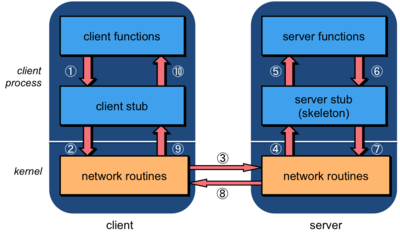
\includegraphics[width=0.5\textwidth]{figuras/How-RPC-Works.png}
\label{fig:rpc}
\caption{RPC fluxo de dados. (refazer)}
%( https://www.cs.rutgers.edu/~pxk/416/notes/15-rpc.html )
\end{figure}

Ainda segunda a especificação do RPC \cite{rfc1831:rpc}(???), há alguns aspectos importantes onde as chamadas remotas se diferem das chamadas locais:

\begin{itemize}
\item Tratamento de erros: Falhas no servidor remoto ou da rede devem ser tratadas quando usando uma RPC.

\item Variáveis globais e efeitos colaterais: Uma vez que o servidor não tem acesso ao espaço de endereço do cliente, argumentos ocultos não podem ser passados como variáveis globais ou retornados como efeitos colaterais.

\item Desempenho: Chamadas remotas geralmente operam uma ou mais ordens mais lentos do que chamadas de procedimentos locais

\item Autenticação: Uma vez que as chamadas remotas pode ser transportadas através de redes insegurar, autenticação pode ser necessário. Autenticação previne uma entidade de se passar por outra e executar chamadas indevidas.

\end{itemize}

\subsection{Limitações}

Diferentes implementações de RPC são geralmente mutualmente incompatíveis. Assim sendo, o uso de uma implementação específica provavelmente resultará na dependência da implementação do fornecedor. Esse tipo de incompatibilidade entre diferentes implementações implica em um diverso número de funcionalidades, suportando inúmeros protolos de rede e diferentes sistemas de arquivos.
%( https://www.eukhost.com/blog/webhosting/remote-procedure-call-rpc/ )

\citeonline{rpc-limitations} aponta diversas limitações técnicas e de desempenho encontradas geralmente em implementações de RPC's. Dentre estas limitações, se destacam:

\begin{itemize}

\item Organização dos parâmetros \textit{Encontrar outro}: Para organizar os parâmetros, o cliente precisa conhecer o número e o tipo dos parâmetros exatos. Como não existe uma padrão bem definido, a estruturação dos parametros podem varias entre diferentes implementações, o cliente não tem facilidade de constatar o número de parâmetros que existem ou os tipos desses parâmetros.

\item Falta de paralelismo: Com RPC, em um determinado momento, ou o servidor ou o cliente esta ativo. Como cliente e servidor são co-rotinas, a pratica de paralelismo presente em outros modelos de comunicação, não é possível de ser implementada.

\item Falta de transmissão: Em banco de dados, um cliente solicita a um servidor que execute a operação para procurar dados no banco de dados que atendam a algumas condições. Usando o modelo do RPC, um servidor deve esperar até que todas as informações sejam encontradas antes de responder. Caso a operação de busca em todos os dados seja demorada, o cliente permanece ocioso por algum tempo, esperando que a última tupla seja pesquisada.

\end{itemize}

\section{Simple Object Access Protocol}\label{sec:soap}

Simple Object Access Protocol (SOAP) é um protocolo para troca de mensagens em ambientes descentralizados e distribuídos. \citeonline{soap2000} define o SOAP como 
um protocolo baseado em XML que consiste em três partes: um envelope que defina um \textit{framework} para descrever o que há mensagem e como processar seu conteúdo, um conjunto de regras de codificação para expressar instâncias de tipos de dados definidos por uma aplicação, e uma convenção para para representar chamadas remotas e suas respostas.

Para \citeonline{soap-smartbear}, o SOAP é um protocolo de acesso a serviços baseados em padrões que existe por um tempo e utiliza-se de todos os benefícios do uso a longo prazo. Originalmente desenvolvido pela Microsoft, ele pode não ser tão simples quanto o acrônimo sugere.

\citeonline{soap-tech-target} argumenta que o SOAP pode ser considerado parecido com as Chamadas de Procedimento Remoto (RPC), porém eliminando alumas das complexidades frequentemente encontradas nas implementações de RPC's. Utilizando o SOAP, é possível chamar serviços de outras aplicações, que estão sendo executadas em qualquer \textit{hardware}, independente do sistemas operacional ou linguagem de programação.

Embora a especificação do SOAP tenha evoluído para longe da necessidade de acessar objetos, como ocorre com com as Chamadas de Procedimentos Remoto, existe ainda convenções para o encapsulamento e envio de chamadas RPC utilizando uma representação uniforme de chamadas e repostas. Definindo um padrão para o mapeamento das chamadas RPC para SOAP torna-se possível para infraestrutura traduzir as invocações de serviços em mensagens com o protocolo SOAP em tempo de execução, sem a necessidade de redesenhar todo o serviço Web presente na plataforma \cite{soap-microsoft}.

\begin{figure}[htbp]
\centering
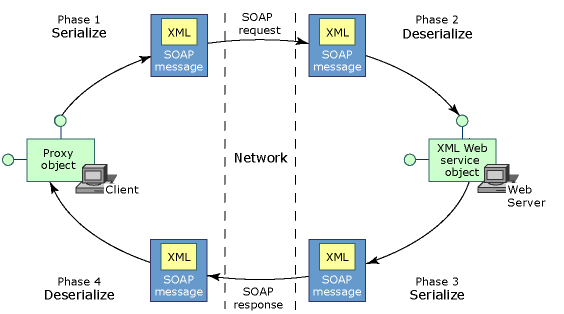
\includegraphics[width=1\textwidth]{figuras/soap-st.png}
\label{fig:soap}
\caption{SOAP fluxo de dados. (refazer)}
\author{https://msdn.microsoft.com/en-us/library/x05s00wz(v=vs.80).aspx}
\end{figure}

\pagebreak

% LER https://imasters.com.br/artigo/4379/web-services/protocolo-de-transporte-padrao-soap?trace=1519021197&source=single

\citeonline{soap-benefits} assinala que SOAP é um protocolo que define uma gramática XML especializada, que padroniza o formato das estruturas das mensagens. As mensagens são, por outro lado, o método fundamental de troca de informações entre os Web Sevices e os seus consumidores. Ao utilizar XML para codificar mensagens o SOAP nos dá alguns benefícios:

\begin{itemize}
\item Permite a comunicação entre sistemas protegidos por \textit{firewalls}, sem precisar abrir portas adicionais e possivelmente não seguras
\item XML pode ser facilmente lido por humanos, sendo portanto, mais fácil de entender e eliminar erros.
\item Os dados do SOAP são estruturados usando XML. Portanto, as mensagens podem ser compreendidas por quase todas as plataformas de hardware, sistemas operacionais e linguagens de programação.
\item Pode ser usado, potencialmente, em combinação com vários protocolos de transporte de dados, como HTTP, SMTP e FTP.
\item O SOAP mapeia satisfatoriamente para o padrão de solicitação / resposta do HTTP.
\end{itemize}

\subsection{Limitações}

\citeonline{soap-limitations} explica que tecnologias de metadados abertas, como o XML, podem fornecer um grande ganho de usabilidade, mas o sucesso dessas tecnologias exige que seu uso não degrada o desempenho de forma irracional.O XML é extremamente robusto, no entanto, seu o uso pode afetar negativamente o desempenho do SOAP nas seguintes áreas:

Velocidade de codificação e decodificação. A conversão de dados de binário para ASCII e vice-versa é o principal custo de desempenho do XML. O uso de um protocolo baseado em texto também impede a aplicação de otimizações disponíveis para protocolos binários quando a comunicação ocorre entre sistemas homogêneos.

Tamanho da mensagem. Para XML, um fator de expansão de 6-8 vezes em relação aos dados binários originais não é incomum. Mediu a expansão em 4 a 10 vezes e descobriu que o tamanho da representação de dados do SOAP é tipicamente cerca de 10 vezes o tamanho da representação binária equivalente. Este tamanho substancialmente maior pode resultar em maiores custos de transmissão de rede e latência aumentada.

Como é possível notar, as maiores limitações encontradas na utilização do SOAP como modelo de comunicação estão relacionadas a estruturação usando XML. Embora esse formato padrão de mensagens tnha trazido vantagens em relação a tecnologias anteriores ao SOAP, ele também trouxe uma série de barreias conforme sua popularidade foi crescendo. \textit{A necessidade buscar alternativas para superar esses problemas  foi crescente, e o mercado encontro novos formatos foram aparecendo, tendo como destaque o JSON}

\section{REpresentational State Transfer}\label{sec:rest}

Representational State Transfer (REST) é um \textit{design} de arquitetura baseado em um conjunto de princípios que descrevem como os recursos em rede são definidos e abordados. Estes princípios foram descritos pela primeira vez em 2000 por Roy Fielding como parte de sua dissertação de doutorado \cite{rest-intro}.

%http://www.servicearchitecture.com/articles/webservices/representational_state_transfer_rest.html

\citeonline{programmableweb-rest-losing} assinala que a adoção do REST (REpresentational State Transfer) como o método predominante para construir APIs públicas tem ofuscado qualquer outra tecnologia ou abordagem nos últimos anos. Embora várias alternativas (principalmente SOAP) ainda estejam presentes no mercado, adeptos do modelo SOA, descrito da seção 2.4,  para construção de aplicações tomaram uma posição definitiva contra eles e optaram por REST como sua abordagem e JSON como seu formato de mensagem .

Segundo \citeonline{rest-book-intro:61}, REST é um padrão de operações de recursos que emergiu como a principal alternativa ao já antigo SOAP para o design de serviços em aplicativos Web 2.0. Considerando que a abordagem tradicional baseada em SOAP para Web Services usa objetos remotos completos com invocação de método remoto e funcionalidade encapsulada, o REST trata apenas de estruturas de dados e da transferência de seu estado. A simplicidade do REST, juntamente com seu ajuste natural sobre o HTTP, contribuiu para o seu status como um método de escolha para aplicativos da Web 2.0 para expor seus dados.

\subsection{Restrições}

As restrições do REST são regras desenhadas para estabelecer as caracteristicas distinctas da arquitetura REST. Cada restrição é uma decisão de projeto pré-determinada que pode ter impactos positivos e negativos. A intenção é que os aspectos positivos de cada restrição equilibrem os negativos para produzir uma arquitetura geral que se assemelhe à Web.

Uma arquitetura que elimina uma restrição REST, geralmente é considerada como não mais conforme ao REST. Isso exige que as decisões sejam tomadas para entender os potenciais \textit{trade-offs} quando se desviam deliberadamente da aplicação de restrições REST. 

A primeira restrição estabelecida é a da arquitetura \textbf{cliente-servidor}, descrita na Seção 2.2. A separação de responsabilidades é o princípio por trás das restrições cliente-servidor. Ao separar as responsabilidades da interface do usuário com as responsabilidades de armazenamento de dados, melhoramos a portabilidade da interface do usuário em várias plataformas e melhoramos a escalabilidade, simplificando os componentes do servidor. Talvez o mais importante para a Web, no entanto, é que a separação permite que os componentes evoluam de forma independente, apoiando assim o requisito de escalabilidade da Internet de múltiplos domínios organizacionais \cite{rest-thesis}

Em seguida, adicionamos uma restrição à interação cliente-servidor: a comunicação deve ser totalmente \textbf{stateless}, ou seja, independente de estado, de modo que cada solicitação do cliente para O servidor deve conter todas as informações necessárias para entender o pedido e não pode tirar proveito de nenhum contexto armazenado no servidor. O estado da sessão é, portanto, mantido inteiramente no cliente \cite{rest-thesis}.

Essa restrição induz as propriedades de visibilidade, confiabilidade e escalabilidade. A visibilidade é melhorada porque um sistema de monitoramento não precisa olhar além de um único dado de solicitação para determinar a natureza completa da solicitação. A confiabilidade é melhorada porque facilita a tarefa de recuperação de falhas parciais. A escalabilidade é melhorada porque não ter que armazenar o estado entre solicitações permite que o componente do servidor rapidamente libere recursos e simplifica ainda mais a implementação porque o servidor não precisa gerenciar o uso de recursos em todos os pedidos.

A restrição de \textbf{cache} foi criada para melhorar a eficiência da rede. Ela exigem que os dados dentro de uma resposta a uma solicitação sejam rotulados de forma implícita ou explícita como cacheáveis ou não armazenáveis em cache. Se uma resposta for armazenada em cache, um cache do cliente terá o direito de reutilizar esses dados de resposta para solicitações equivalentes posteriores.

A vantagem de adicionar restrições de cache é que eles têm o potencial de eliminar parcial ou totalmente algumas interações, melhorar a eficiência, escalabilidade e desempenho percebido pelo usuário, reduzindo a latência média de uma série de interações. O \textit{trade-off}, no entanto, é que um cache pode diminuir a confiabilidade se os dados obsoletos dentro do cache diferirem significativamente dos dados que teriam sido obtidos se a solicitação fosse enviada diretamente para o servidor.

A característica central que distingue a arquitetura REST de outros estilos baseados em rede é a ênfase em uma \textbf{interface uniforme} entre os componentes. Ao aplicar o princípio de engenharia de software de especialização/generalização para a interface do componente, a arquitetura geral do sistema é simplificada e a visibilidade das interações é melhorada. As implementações são dissociadas dos serviços que eles fornecem, o que incentiva a evolução independente. O trade-off, no entanto, é que uma interface uniforme degrada a eficiência, uma vez que a informação é transferida em uma forma padronizada e não específica para as necessidades de uma aplicação.

Para obter esta interface uniforme, são necessárias várias restrições arquitetônicas para orientar o comportamento dos componentes. REST é definido por quatro restrições de interface: identificação de recursos; Manipulação de recursos através de representações; Mensagens auto-descritivas; E, hipermídia como motor do estado da aplicação.

A fim de melhorar o comportamento dos requisitos de escalamento, o REST também implementa restrições de \textbf{sistema em camadas}. O sistema em camadas permite que uma arquitetura seja composta de camadas hierárquicas ao restringir o comportamento dos componentes, de modo que cada componente não possa "ver" além da camada imediata com a qual eles estão interagindo. Ao restringir o conhecimento do sistema a uma única camada, colocamos um limite na complexidade geral do sistema e promovemos a independência do componentes. As camadas podem ser usadas para encapsular serviços legados e para proteger novos serviços de clientes legados, simplificando componentes e movendo funcionalidades raramente usadas para um intermediário compartilhado. Os intermediários também podem ser usados para melhorar a escalabilidade do sistema ao permitir o balanceamento de carga de serviços em várias redes e processadores.

A principal desvantagem dos sistemas em camadas é que eles adicionam sobrecarga e latência ao processamento de dados, reduzindo o desempenho perceptível pelo usuário. Para um sistema baseado em rede que suporta restrições de cache, isso pode ser compensado pelos benefícios do armazenamento em cache compartilhado em intermediários.

A ultima restrição que o REST implementa é a restrição de \textbf{código por demanda}. O REST permite que a funcionalidade do cliente seja estendida baixando e executando o código na forma de \textit{applets} ou \textit{scripts}. Isso simplifica os clientes, reduzindo o número de recursos necessários para serem pré-implementados. Permitir que os recursos sejam baixados após a implantação, melhora a extensibilidade do sistema, no entanto, também reduz a visibilidade e, portanto, é apenas uma restrição opcional dentro do REST.

%https://www.ics.uci.edu/~fielding/pubs/dissertation/rest_arch_style.htm
%http://whatisrest.com/rest_constraints/index

\subsection{Modelo de Maturidade de Richardson}

%https://restfulapi.net/richardson-maturity-model/
%https://martinfowler.com/articles/richardsonMaturityModel.html
%http://restcookbook.com/Miscellaneous/richardsonmaturitymodel/
%https://dzone.com/articles/building-hateoas-hypermedia


O Modelo de Maturidade de Richardson, é um modelo criado por Leonard Richardson que descreve os requisitos necessários para o desenvolvimento de uma API REST bem estruturada e compatível com as restrições definidas pela arquitetura REST. Quanto melhor a API adere as restrições citadas na sessão anterior, melhor será pontuada. O  modelo de Richardson descreve 4 níveis (0-3), onde o nível 3 designa uma API verdadeiramente \textit{RESTful}. Richardson usou três fatores para decidir a maturidade de uma API: URI (Uniform Resource Identifiers), métodos HTTP e HATEOAS (Hypermedia). Quanto mais uma API emprega essas tecnologias, mais madura ela é categorizada.

\begin{figure}[htbp]
\centering
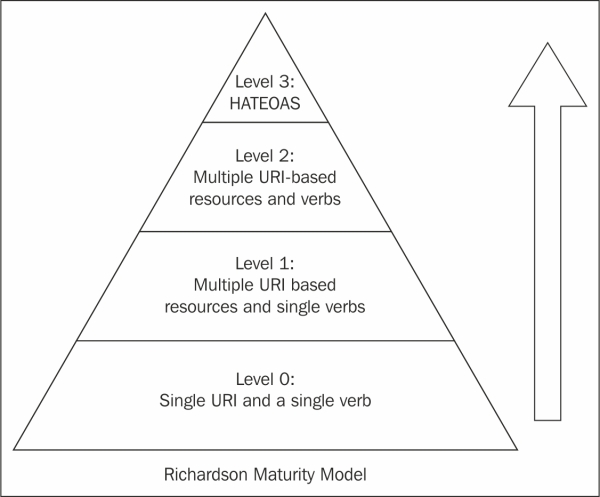
\includegraphics[width=0.5\textwidth]{figuras/rest-maturity-model.jpg}
\label{fig:rest-maturity-model}
\caption{Modelo de maturidade de Richardson. (refazer)}
\author{}
\end{figure}

\begin{itemize}
\item Nível 0: O ponto de partida para o modelo é usar HTTP como um sistema de transporte para interações remotas, mas sem usar nenhum dos mecanismos da web. Essencialmente, o que você está sendo feito é utilizar o HTTP como um mecanismo de tunelamento para seu próprio mecanismo de interação remota, geralmente com base em Chamadas de Procedimento Remotas. 

É como se estivesse sendo chamado funções, porém através do uso do HTTP. Todos serviços são centralizados em um único \textit{endpoint}, ou seja, todas as solicitações são feitas em uma única URI.

\item Nível 1: Quando uma API faz a distinção entre recursos diferentes, pode se considerar que atingiu o nível 1. Esse nível usa vários URIs, onde cada URI é o ponto de entrada para um recurso específico. Ainda assim, esse nível usa apenas um único método, como o POST.

\item Nível 2: Esse nível indica que a API deve usar as propriedades do protocolo para lidar com escalabilidade e falhas. Não é recomendado que se use um único método POST para todas as chamadas, mas faça uso do GET quando estiver solicitando recursos e use o método DELETE quando desejar excluir recursos. Além disso, o uso dos códigos de resposta do protocolo de aplicação também é recomendado. Não deve ser usando, por exemplo, o código 200 (OK) quando algo der errado.

\item Nível 3: O nível três de maturidade faz uso de todos os três fatores, isto é, URIs, métodos HTTP e HATEOAS. Esse é o nível em que a maioria das APIs menos implementam e pois não seguem o princípio de HATEOAS.

HATEOAS (Hypermedia as the Engine of Application State) é uma abordagem para a construção de serviços REST, onde o cliente pode descobrir dinamicamente as ações disponíveis em tempo de execução. Todo o cliente deve exigir para começar é um URI inicial e um conjunto de tipos de mídia padronizados. Uma vez que carregou o URI inicial, todas as futuras transições de estado da aplicação serão conduzidas pelo cliente selecionando as escolhas fornecidas pelo servidor.

Não seguir essa abordagem não é necessariamente ruim. Há alguns bons argumentos a serem feitos a favor e contra a utilização de HATEOAS. Enquanto, por um lado, torna as APIs fáceis de descobrir e usar, que geralmente vem ao custo de mais tempo e esforço de desenvolvimento.

\end{itemize}

\subsection{Limitações}

Contudo, com a evolução e o aumento da complexidade das APIs, a comunicação via o protocolo REST vem se mostrando muitas vezes inviável pois sua implementação trás como consequências alguns problemas estruturais como:

\begin{itemize}

\item A necessidade de executar múltiplas requisições entre o cliente e o servidor a fim de obter objetos complexos e com atributos aninhados  Para aplicações móveis operando em condições variáveis de rede, essas múltiplas viagens de ida e volta são indesejáveis, pois geram atrasos e maior tráfego na rede \cite{graph-intro}.

\item A prática de \textit{over-fetching}, ou seja, quando o cliente busca alguma informação do servidor e a resposta contém mais informação que o cliente precisa. Esse tipo de problema acarreta no uso desnecessário de recursos de comunicação  \cite{efficient-data-communication}.

\item O versionamento da API, que ocorre quando há alterações significativas na API, sujeitas a quebra de código nos clientes consumidores. Essa prática pode ser extremamente penosa se a API é usada por uma grande massa de clientes que não são facilmente atualizados \cite{api-versioning}.

\end{itemize}

\section{Arquiteturas baseadas em JSON/Graphs}\label{sec:graph}

Recentemente, um novo design de arquitetura vem ganhando espaço, preenchendo algumas lacunas que arquiteturas anteriores deixaram. Lideradas pelo Facebook com seu GraphQL e Netflix com o Falcor, esta nova arquitetura da um passo para trás comparando-se ao REST, atingindo apenas o nivel 0 no Modelo de Maturidade de Richardson. 

Os principais problemas que essa arquitetura ajuda a resolver são: A dependência das aplicações cliente nos servidores, eliminando a necessidade do servidor de ter que manipular as informações ou o tamanho da resposta; A necessidade de executar diversas requisições para acessar os dados exigidos por uma \textit{view}; Melhorar a experiência de desenvolvimento \textit{frontend}, pois existe uma relação próxima entre os dados necessários à interface da aplicação e a forma como um desenvolvedor pode expressar uma descrição desses dados para a API. O presente trabalho irá apenas focar no GraphQL como representante das arquiteturas baseadas em JSON/Graph.

GraphQL é uma linguagem de consulta criada pelo Facebook em 2012, que fornece uma interface comum entre o cliente e o servidor para manipulação e busca de dados. GraphQL utiliza de um sistemas chamado \textit{cliente-specified queries}, onde o o formato de resposta de uma requisição é definida pelo cliente. \citeonline{graphQl-overview} afirma que uma vez que a estrutura de dados não é codificada, como nas APIs tradicionais, a consulta de dados do servidor se torna mais eficiente para o cliente.

Consultas utilizando GraphQL sempre retornam apenas o que foi pré definido pela requisição, fazendo suas respostas sempre serem previsíveis. As consultas com GraphQL acessam não apenas as propriedades de um único recurso, mas também seguem as referências entre eles. Enquanto as APIs REST típicas exigem o carregamento de múltiploas URLs, as APIs GraphQL obtêm todos os dados que precisam em uma única requisição.

Adicionar novos campos ou tipos á uma API GraphQL não afeta nenhuma consulta ou funcionalidade já existente. Campo não mais utilizados podem ser obsoletos e ocultos de ferramentas de mapeamento. Ao usar uma única versão em evolução, as APIs GraphQL dão as aplicações acesso contínuo a novos recursos e encorajam um código de servidor mais limpo e mais sustentável.

\subsection{Operações}

Existem três tipos de operações modeláveis com GraphQL:

\begin{itemize}
\item Query: Uma consulta de somente leitura
\item Mutation: Uma escrita seguira por consulta
\item Subscription – Uma requisição de longa duração que obtém dados em resposta a eventos disparados pelo servidor.
\end{itemize}

Uma Query em GraphQL é uma maneira de obter dados de uma maneira somente de leitura em uma API GraphQL. De uma maneira geral, GraphQL é se baseia em consultar campos específicos em objetos. Isso significa que a consulta tem exatamente o mesmo formato que a resposta. Isso é essencial para GraphQL, porque a resposta é sempre previsível, e o servidor sabe exatamente quais os campos que o cliente está pedindo.

Como GraphQL não se limita apenas em consultas de dados, as APIs também podem implementar operações para criar, atualizar e destruir dados. Para esses tipos de operações, o GraphQL usa o termo Mutations. As Mutations são uma maneira de alterar dados em seu servidor. É importante notar que as \textit{mutations} consistem em uma alteração seguida de uma busca do dado que acabou de ser alterado, tudo em uma única operação.

Os aplicativos em tempo real precisam de uma maneira de enviar dados do servidor. As subscriptions permitem que aplicações publiquem eventos em tempo real através de um servidor de assinaturas GraphQL.
Com o modelo de subscriptions baseado em eventos no GraphQL - muito parecido com as quaries e mutations - um cliente pode dizer ao servidor exatamente quais dados devem ser enviados e como esses dados devem ser encontrados. Isso leva a menos eventos rastreados no servidor e notificados para o cliente.

\subsection{Schemas e Tipos}

%https://facebook.github.io/graphql

O sistema de tipos do GraphQL descreve as capacidades de um servidor GraphQL e é usado para determinar se uma consulta é válida. O sistema de tipos também descreve os formatos de entrada de variáveis de consulta para determinar se os valores fornecidos em tempo de execução são válidos. As capacidades do servidor GraphQL são referidas como \textit{schema} do servidor. Um \textit{schema} é definido baseado nos tipos que ele suporta.

Cada servidor GraphQL define um conjunto de tipos que descrevem completamente o conjunto de dados possíveis que você pode consultar nesse servidor. Então, quando as consultas chegam, elas são validadas e executadas contra os \textit{schemas}. O \textit{schema} descreverá quais campos o servidor pode responder e quais tipos de objetos as respostas irão conter. A informação de tipo é muito importante para o GraphQL e o cliente pode assumir de forma segura que o servidor retornará tipos consistentes de objetos para o mesmo campo.

A unidade fundamental de qualquer \textit{schema} GraphQL é o tipo. Existem oito formatos de tipos suportados no GraphQL. O tipo mais básico é o \textit{\textbf{Scalar}}. Um campo do tipo \textit{Scalar} representa um valor primitivo, como uma \textit{string} ou um número inteiro. Muitas vezes, as respostas possíveis para um campo  do tipo \textit{Scalar} são enumeráveis. O GraphQL oferece um tipo \textit{\textbf{Enum}} nesses casos, onde o tipo especifica o espaço de respostas válidas. Campos do tipo \textit{\textbf{Object}} definem um conjunto de campos, onde cada campo é outro formato, permitindo a definição de hierarquias de tipos arbitrários. O GraphQL suporta dois tipos abstratos:  \textit{\textbf{Interfaces}} e  \textit{\textbf{Unions}}.

Todos os tipos até agora são considerados nulos e singulares, por exemplo,  uma \textit{string} retorna um valor nulo ou singular. O sistema de tipo pode querer definir que ele retorna uma lista de outros tipos; O tipo \textit{\textbf{List}} é fornecido por esse motivo e envolve outro tipo. Da mesma forma, o tipo \textit{\textbf{Non-Null}} envolve outro tipo e indica que o resultado nunca será nulo.

Finalmente, muitas vezes é útil fornecer estruturas complexas como entradas para consultas GraphQL; o tipo \textit{\textbf{Input Object}} permite que o \textit{schema} defina exatamente quais dados são esperados do cliente nessas consultas.


\subsection{Autorização}

Segundo \citeonline{rfc2977}, Autorização é o ato de determinar se um direito particular, como acesso a algum recurso, pode ser concedido à uma determinada credencial. Nos sistemas de informação multiusuários, o administrador do sistema define quais usuários podem ter acesso ao sistema e quais são os privilégios de uso.

Normalmente o GraphQL não controla diretamente o controle de acesso, em vez disso, delega essa responsabilidade para a camada de lógica de negocio da aplicação. 


\subsection{Caching}

De acordo com \citeonline{graph-cache}, consultas de dados através da internet podem ser lentas e custosas, e por esse motivo, a capacidade de armazenar em cache e reutilizar os recursos obtidos anteriormente é um aspecto crítico da otimização para o desempenho.

\begin{figure}[htbp]
\centering
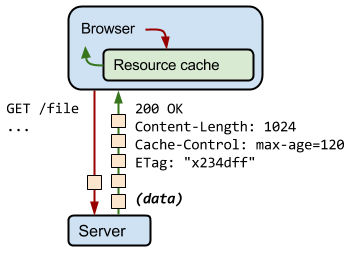
\includegraphics[width=0.5\textwidth]{figuras/cache-http.png}
\label{fig:cache-graph}
\caption{HTTP Caching. (refazer)}
\author{https://developers.google.com/web/fundamentals/performance/optimizing-content-efficiency/http-caching}
\end{figure}

Em uma API baseada em \textit{end-points}, os clientes podem usar o armazenamento em cache do protocolo HTTP para evitar buscas desnecessárias identificando quando dois recursos são iguais. A URL nessas APIs é o identificador globalmente exclusivo que o cliente pode aproveitar para criar um cache. No GraphQL, porém, não existe uma primitiva semelhante a uma URL que forneça esse identificador globalmente exclusivo para um determinado objeto. Entretanto, existem várias práticas que podem ser aplicadas a um servidor GraphQL para atingir o mesmo objetivo.

Um padrão possível para isso é reservar um campo, como id, para ser o identificador globalmente exclusivo. Da mesma forma que os URLs de uma API baseada em recursos fornecem uma chave globalmente exclusiva, o campo id neste sistema fornece uma chave globalmente única. Outra abordagem possível funcionaria de forma semelhante à ao padrão usada nas APIs baseadas em \textit{end-points}. O texto da consulta em si pode ser usado como identificador globalmente exclusivo. 


\subsection{Limitações}

Segundo aponta \citeonline{graph-limitation}, uma ameaça importante que o GraphQL facilita são os ataques de negação de serviço. Um servidor GraphQL pode ser atacado com consultas excessivamente complexas que irão consumir todos os recursos do servidor. Esse tipo de ataque não é específico do GraphQL, mas é preciso um cuidado redobrado para evitar-los.

Há entretanto, alguns procedimento que se implementados, podem mitigar a ameaça de negação de serviço. É possível fazer uma análise de custos na consulta com antecedência e impor um certo tipo de limites na quantidade de dados que uma requisição pode consumir. Também é possível implementar um tempo limite para que requisições que levam muito tempo para serem resolvidas, sejam excluídas da fila de execução .

%https://arxiv.org/pdf/1701.00626.pdf


  % ----------------------------------------------------------
% Protocolos de comunicaçào
% ----------------------------------------------------------
\chapter[Estudo de Caso]{Estudo de Caso}\label{cap:estudo}
%\addcontentsline{toc}{chapter}{Protocolos de Comunicação}
% ----------------------------------------------------------

Para obter um exemplo do mundo real, um estudo de caso foi projetado com base em uma aplicação de WMS (\textit{Warehouse Management System}). \citeonline{wms-definition} explica que um sistema de WMS é um software que auxilia as operações do dia-a-dia em um armazém. Os sistemas WMS permitem o gerenciamento centralizado de tarefas, como o rastreamento de níveis de inventário e locais de estoque. Tais sistemas WMS podem ser um aplicativo independente ou parte de um sistema de ERP.

Com o intuito de realizar consultas relevantes, foi modelado um esquema contendo seis entidades capazes de representar consultas reais, e ainda produzirem informações pertinentes para comparar o desempenho dos protótipos. A construção das APIs seguiram os princípios do ciclo tradicional do desenvolvimento de \textit{software}, portanto a modelagem foi elaborada antes do início da implementação das APIs. Isso assegura que nenhuma decisão de tecnologia tenha afetado a modelagem das entidades.

A modelagem da figura \ref{fig:modelagem}, representa o gerenciamento de um armazém com capacidade de armazenar diversos itens. Os itens são dispostos em \textit{pallets}, e alocados em endereços dentro do armazém. Como pode ser observado na figura \ref{fig:rack}, os endereços do armazém são formados a partir de uma combinação de três dimensões: \textbf{Prateleira}, \textbf{Linha} e \textbf{Nível}. Cada combinação dessas três propriedades é capaz de alocar \textit{pallets}, que por sua vez podem conter diversas unidades de um mesmo item.

\begin{figure}[htbp]
\centering
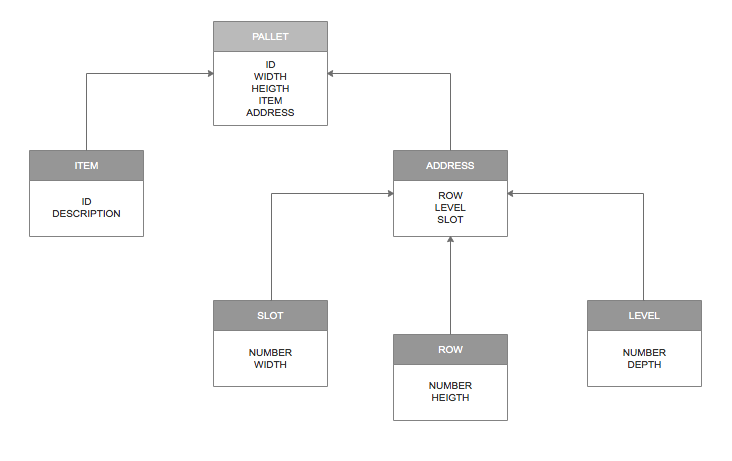
\includegraphics[width=0.9\textwidth]{figuras/model.png}
\caption{Modelagem WMS}
\label{fig:modelagem}
\legend{Fonte: Autor}
\end{figure}

Imagine um item de código 22B12, por exemplo, que representa um dado produto X. Este produto é disposto em um \textit{pallet} com capacidade de armazenar 30 unidades do item 22B12. O armazém é composto por 26 prateleiras, sequenciadas de 'A' a 'Z'. Cada prateleira possui 2 linhas de profundidade e 3 níveis de altura. Um \textit{pallet} com o código 001 contém 30 unidade do item 22B12, e precisa ser alocado dentro armazém, para isso é utilizado um sistema de códigos envolvendo as 3 dimensões do armazém.

\begin{figure}[htbp]
\centering
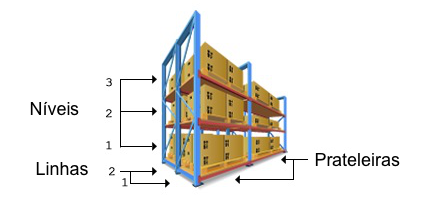
\includegraphics[width=0.7\textwidth]{figuras/rack.png}
\caption{Diagrama de dimensões do armazém}
\legend{Fonte: \citeonline{wms-rack}}
\label{fig:rack}
\end{figure}

Desta forma, 60 unidades do item 22B12 estão dispostos em dois \textit{pallets}(001, 002) existentes no armazém, e cada um dos \textit{pallets} será destinado a um endereço. O \textit{pallet} 001 será alocado na terceira prateleira, no segundo nível e na primeira linha. Após a formação do endereço, o \textit{pallet} 001 estará localizado no endereço C0201, prateleira C, nível 02 e linha 01.

Baseado em um sistema de WMS, dois protótipos de APIs serão implementados para uma análise. A primeira API será implementada seguindo as melhores práticas do \textit{design} do REST, descritas na sessão \ref{sec:rest}. A segunda será desenvolvida utilizando o GraphQL, e o seu desempenho será comparado com a API REST.

\section{Hipóteses} \label{sechHipóteses}

As hipóteses na diferença de desempenho entre as APIs derivaram dos fundamentos teóricos. Elas baseiam-se no entendimento de que os protocolos utilizados possibilitam a implementação de uma combinação de técnicas afim de afetar positivamento o desempenho da API. Portanto, ambas as implementações devem ter as mesmas propriedades, seguindo suas melhores práticas, modelos de maturidade e documentação.

As hipóteses deste trabalho são: 

\begin{enumerate}[label=\alph*)]
\item O tamanho da resposta será menor utilizando GraphQL;
\item O tempo de resposta será menor utilizando GraphQL;
\item O tempo de utilização da CPU será menor utilizando REST;
\item O consumo de memória será menor Utilizando REST;
\end{enumerate}

Com o propósito de validar as hipóteses definidas, foram determinadas duas perguntas que envolvessem todas as entidades. Para cada pergunta existe apenas uma resposta correta e sua lógica é baseada em campos das estruturas de dados de retorno.

\textbf{Questão 1}: Qual item ocupa a maior quantidade de \textit{pallets} alocados no armazém?

\textbf{Questão 2}: O item com o código 22B12 está armazenado em quais endereços?

Desta forma, buscas serão realizadas tanto na API REST quanto na API GraphQL afim de recuperar as informações necessárias para a formulação das respostas. Para realizar estas buscas, medir o desempenho das APIs processando suas respostas e compara-los, algumas ferramentas foram utilizadas durante este trabalho. Estas ferramentas estão descritas na sessão \ref{sec:ferramentas}.

\section{Ferramentas utilizadas} \label{sec:ferramentas}

A escolha das ferramentas a serem usadas na implementação foi uma das partes mais importantes no planejamento do estudo de caso. Foi necessário pensar em uma especificação que apresentasse uma curva rápida de aprendizagem, um fluxo de execução replicável e independente de plataforma, e uma documentação madura em relação à implementação das APIs.

As APIs foram escritas na linguagem de programação JavaScript, utilizando a especificação do ECMAScript 5. Foi escolhida esta linguagem devido ao fácil acesso a boas ferramentas para construção de serviços Web, como o Node.js. Node.js é uma plataforma para desenvolvimento de servidores Web utilizando JavaScript e o V8 JavaScript Engine. Assim, com Node.js pode-se criar uma variedade de aplicações Web utilizando código em JavaScript \cite{node-definition}.

\subsection{Ferramentas servidor}

Node.js dispõe de inúmeros recursos e ferramentas que possibilitam a construção de APIs. Mesmo assim, o ecosistema de bibliotecas no Node.js conta com ferramentas que simplificam ainda mais a construção de aplicações para servidores Web. Abaixo são citadas algumas bibliotecas que foram utilizadas para desenvolver tanto a API REST quando a API GraphQL. 

\subsubsection*{Expess.js}

Express.js é um \textit{framework} para Node.js extremamente flexível, que fornece um conjunto robusto de ferramentas para a construção de aplicações Web e Móveis. Conta com um robusto sistema de roteamento, facilitando o desenvolvimento de APIs. O Express.js fornece uma fina camada de abstração nas principais funcionalidades do Node.js, sem sobrepor seus recursos.

Nos protótipos desenvolvidos para executar o experimento, o Express.js atua como um \textit{middleware}, gerenciando as rotas e delegando a responsabilidade de interpretação das requisições para os \textit{Controllers} na API REST e para os \textit{Resolvers} na API GraphQL.

O código \ref{lst:load-rest} ilustra como os \textit{Controllers} enviam as informações da requisição para o modelo, que é o responsável na API REST em executar as consultas no banco de dados. No exemplo abaixo, o trecho de código é o responsável por retornar um \textit{Item} baseado no \textup{id} recebido como parâmetro da requisição. É possível observar que na linha 2 o modelo da entidade \textit{Item} é importado para ser utilizado no \textit{Controller}, e na linha 8, o método \textup{get}, cujo a lógica está implementada dentro do modelo, é invocado passando como parâmetro o \textup{id}.

\begin{lstlisting}[escapeinside={(*}{*)}, numbers=left, caption={Controller para carregar um item}, label=lst:load-rest,language=JavaScript]
//item.controller.js
import Item from '../models/item.model';

/**
 * Load item and append to req.
 */
function load(req, res, next, id) {
  Item.get(id)
    .then((item) => {
      req.item = item;
      return next();
    })
    .finally(e => next(e));
}

\end{lstlisting}

Já o código \ref{lst:express-graph} mostra como o Express.js gerencia a requisição recebida via método GET, e delega a responsabilidade para o \textup{schema.js}, onde está contida a lógica para a interpretação dos parâmetros da requisição, e retorna um objeto JSON com a devida resposta.

\begin{lstlisting}[escapeinside={(*}{*)}, numbers=left, caption={Expess gerenciando rotas para GraphQL}, label=lst:express-graph,language=JavaScript]
//server.js
import express from 'express';
let app = express();

import schema from './schema.js';

app.get('/', (req, res) => {
    graphql(schema, req.query.query)
    .then((result) => {
        res.send(result);
    });
});

\end{lstlisting}

\subsubsection*{MongoDB}

MongoDB é um banco de dados \textit{open source} que utilizada um modelo de dados orientado a objetos. Ele tem como característica conter todas as informações importantes em um único documento, possuir identificadores únicos universais (UUID), possibilitar a consulta de documentos através de métodos avançados de agrupamento e filtragem, também conhecido como \textit{MapReducers}. Ao invés de usar tabelas e linhas, como os bancos de dados relacionais, o MongoDB usa uma arquitetura baseada em coleções e documentos.


\subsubsection*{Ferramentas clientes}

Algumas ferramentas foram utlizadas para se comportaram como clientes das APIs construídas, e foram responsáveis por executar as consultas nas APIs. O foco deste trabalho não é em cima das aplicação clientes, entretanto é importante conhecê-las pois são elas que invocarão as consultas como também é através delas que algumas métricas serão extraídas. O software Postman será usado fundamentalmente para a execução das buscas nas APIs.

O Postman é uma cadeia completa de ferramentas para desenvolvedores de APIs. Ele é uma ferramenta elegante e flexível usada para construir softwares conectados via APIs, de forma rápida, fácil e precisa.

Ele funciona como uma emulador para execução de consultas em APIs. Com ele é possível executar buscas utilizando qualquer dos métodos do protocolo HTTP, possibilitando personalização tando do corpo quanto dos \textit{headers} das requisições, se preciso. Junto com a resposta da consulta, o Postman traz também informações extremamente relevantes, como tempo que a API levou para responder e o tamanho em bytes contido na resposta. Estas funcionalidades, aliadas com a opção de executar um número personalizável de iterações para cada requisição, será a base para avaliar o desempenho das APIs REST e GraphQL.

\subsection{Ambiente}

A configuração da máquina utilizada para o teste de desempenho local é descrita na Tabela \ref{tab:computers}. As APIs REST e GraphQL foram construídas para responder às requisições recebidas, retornando respostas no formato JSON, a fim de gerar um fator de medição de desempenho da execução dos testes. Para a execução do experimento, apenas os softwares necessários estavam ativos. Portanto, ao executar as buscas, o servidor REST ou GraphQL estará ativo, além do servidor de banco de dados MongoDB, e a aplicação cliente Postman.

\begin{table}[htbp]
    \centering
    \begin{tabular}{| l | l | l |}
        \hline
        \textbf{Item} & \textbf{Computador 1} \\ \hline
        Marca         & Apple                 \\ \hline
        Modelo        & Macbook Air 13"       \\ \hline
        Processador   & Intel Core i5 1.6 GHz \\ \hline
        Memória       & 4 GB 1600 MHz DDR3    \\ \hline
        Disco rígido  & 128 GB SSD            \\ \hline
        Sistema       & macOS Sierra 10.12.6  \\ \hline
    \end{tabular}
    \caption{Especificação da máquina utilizada} \label{tab:computers}
\end{table}

\subsection{Detalhes implementação REST}

O servidor REST consiste em um servidor HTTP escrito em Node.js que recebe as requisições HTTP. Dependendo do método e URL da requisição, roteia-o para o \textit{controller} correspondente. O \textit{controller} faz a consulta na base de dados do MongoDB. Ao realizar o gerenciamento das rotas, o servidor realiza os devidos registros de latência. Após a consulta, a resposta desejada é enviada de volta para o cliente. Esse fluxo acontece em qualquer cenário, independente do número de requisições desejadas.

No presente trabalho, como o objetivo é apenas medir o desempenho de consultas utilizando REST, todas as requisições utilizarão o método HTTP GET. Para as medições da API REST, a aplicação cliente enviará, por exemplo, uma requisição para recuperar todos os itens cadastrados. Como pode ser observado da tabela \ref{tab:rest-url}, é necessário executar uma busca do tipo \textup{/item}, que será interpretada pelo servidor REST, identificando qual é a rota responsável por essa requisição. O servidor consultará a base de dados retornando uma resposta no formato JSON, com todos os itens cadastrados na API. Esse fluxo é ilustrado na figura \ref{fig:rest-uml}

\begin{table}[htbp]
    \centering
    \begin{tabular}{| l | l |}
        \hline
        \textbf{URI} & \textbf{Descrição} \\ \hline
        /item & Consulta lista de itens \\ \hline
        /item/:id & Consulta item pelo id \\ \hline
        /pallet & Consulta lista de pallets  \\ \hline
        /pallet/:id & Consulta pallet pelo id  \\ \hline
        /address & Consulta lista de endereços \\ \hline
        /address/:id & Consulta endereço pelo id \\ \hline
        /slot & Consulta lista de prateleiras \\ \hline
        /slot/:id & Consulta prateleira pelo id \\ \hline
        /row & Consulta lista de linhas \\ \hline
        /row/:id & Consulta linha pelo id \\ \hline
        /level & Consulta lista de nível \\ \hline
        /level/:id & Consulta nível pelo id \\ \hline
    \end{tabular}
    \caption{Servidor REST} \label{tab:rest-url}
\end{table}

\begin{figure}[htbp]
\centering
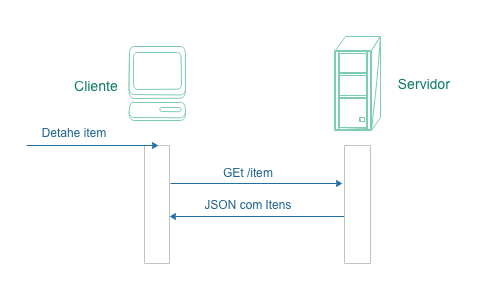
\includegraphics[width=1\textwidth]{figuras/uml-rest.png}
\caption{Fluxo REST}
\label{fig:rest-uml}
\author{fonte: Autor}
\end{figure}

\subsection{Detalhes implementação GraphQL}

O servidor GraphQL foi implementado também usando Node.js. A diferença em comparação com a implementação do servidor REST é que o servidor GraphQL envia todos os pedidos ao seu núcleo, ao invés de rotear as requisições recebidas para vários \textit{controllers} diferentes. O GraphQL analisa a consulta e envia os parâmetros para os \textit{resolvers} responsáveis, localizados nos \textit{schemas}. \textit{Resolvers} são funções definidas para todos os campos no \textit{schema}, cada um retorna os dados para o campo específico. Estas funções são executadas quando os campos correspondentes são consultados e os resultados são retornados na resposta.

\begin{lstlisting}[escapeinside={(*}{*)}, numbers=left, caption=Consulta de itens, label=lst:query-graph, language=JavaScript]]
query RootQuery {
	items {
    	id
    	description
    }
}

\end{lstlisting}

 A consulta ilustrada do trecho de código \ref{lst:query-graph} solicita ao servidor GraphQL a lista a de todos os itens cadastrados na base de dados. Note no trecho de código \ref{lst:response-graph} que a resposta contém apenas os atributos que a consulta requisitou, ou seja, o \textup{id} e a descrição dos itens:

\begin{lstlisting}[escapeinside={(*}{*)}, numbers=left, caption=Listagem dos itens (Validar), label=lst:response-graph, language=JavaScript]]
{
    "data": [
         {
        	"id": 22B12,
            "description": "Flat screen"
        },
        {
        	"id": 21C44,
            "description": "Computer screen"
        },
        {
        	"id": 43F12,
            "description": "Smartphone screen"
        },
    ]
}

\end{lstlisting}

Para recuperar alguma informação na API GraphQL, é necessária realizar uma requisição utilizando o método HTTP GET, passando como parâmetro a consulta desejada. A API irá então processar a consulta, e retornar um objeto JSON como a resposta da requisição. Detalhes deste fluxo esta ilustrado na figura \ref{fig:graph-uml}

\begin{figure}[htbp]
\centering
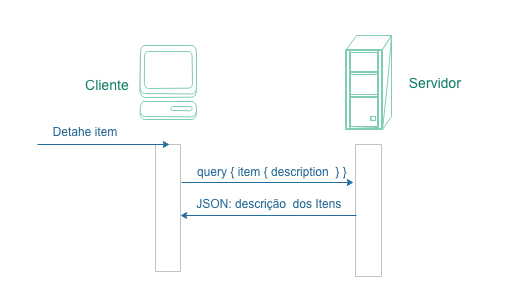
\includegraphics[width=1\textwidth]{figuras/uml-graph.png}
\caption{Fluxo GraphQL}
\label{fig:graph-uml}
\author{fonte: Autor}
\end{figure}

\section{Métricas}\label{sec:metrics}

A fim de comparar as medidas de desempenho de APIs desenvolvidas em REST com APIs desenvolvidas em GraphQL, algumas métricas precisam ser definidas. O desempenho de cada API vai depender de sua implementação, porém, escolhendo as métricas corretas, o efeito da implementação pode ser reduzido. Focando em medições corretas, as diferenças relevantes das APIs podem ser destacadas e melhor ponderadas.

Para o presente trabalho, serão utilizadas quatro métricas diferentes: O tempo de utilização da CPU, Consumo de memória, Tempo de resposta e o Tamanho da resposta. É importante ressaltar que cada métrica foi medida separadamente, para que \textit{logs} e \textit{outputs} pertinentes a uma métrica específica não interfira no resultado das demais.

\subsection*{Tempo de utilização da CPU}

O tempo de utilização da CPU é a quantidade de tempo para o qual uma unidade de processamento central (CPU) foi usada para processar instruções de um programa de computador ou sistema operacional

Esta métrica será extraída através do módulo \textit{process} presente no \textit{core} do Node.Js. A função utilizada será a \textit{process.cpuUsage()} que trás como resultado o tempo gasto por um processo dentro da CPU, calculado pelo sistema operacional. A seguinte fórmula será usada para calcular esta métrica: 

$$ CPU = \frac{\sum\limits_{1}^{n} \Delta cpu}{n} $$

Onde $n$ é o número de CPUs e $\Delta cpu$ é o tempo de uso de CPU pela aplicação, sendo $\Delta cpu = T1 - T2$, em que $T1$ é o tempo final da execução e $T2$ é o tempo inicial. Nos resultados, esta métrica será apresentada na unidade de milissegundos (ms).

\subsection*{Consumo de memória}

O consumo de memória, junto com a utilização da CPU, é uma das medidas mais importantes pois são nesses pontos que observamos o verdadeiro custo computacional por trás da escolha da ferramenta. O consumo de memória é a quantidade de em bytes utilizada pela API, e será medido através da soma da utilização de memória em cada consulta necessária para atender os cenários propostos. A seguinte fórmula será usada para calcular esta métrica: 

$$ Mem = \frac{m}{M}*100 $$

Onde $m$ é a quantidade de memória usada pela aplicação e $M$ é o total de memória. Nos resultados, esta métrica será apresentada na unidade de megabytes.

\subsection*{Tempo de resposta}

É o tempo que cada requisição levou para realizar a consulta. Esse tempo é calculado a partir do início da requisição, até o retorno da resposta completa. No caso da API REST, esta métrica será cumulativa, ou seja, a soma do tempo de todas as requisições necessárias. A seguinte fórmula será usada para calcular esta métrica: 

$$ \Delta t = T1 - T2 $$

Onde $T1$ representa o tempo que a requisição respondeu a consulta, e $T2$ o tempo que foi solicitado a requisição. Nos resultados, esta métrica também será apresentada na unidade de milissegundos (ms).

\subsection*{Tamanho da resposta}

O tamanho da resposta será calculada baseado no tamanho em \textit{bytes} da resposta. Novamente, para a API REST será usada a média das somas de todas as consultas necessárias para obter a resposta desejada. A seguinte fórmula será usada para calcular esta métrica: 

$$ Tam = \sum\limits_{1}^{n} ti $$

Onde $ti$ é o tamanha da resposta de uma requisição, d $n$ é o número total de requisições. Nos resultados, esta métrica será apresentada na unidade de kilobytes.

A figura \ref{fig:my-metrics} mostra como as métricas serão extraídas. A utlização do CPU e o consumo de memória serão medidas utilizando ferramentas do próprio Node.js. Ambas serão medidas via \textit{logs} no código fonte dos protótipos implementados. O tamanho da resposta e o tempo de resposta serão extraídos utilizando a ferramenta Postman, ao final de cada consulta.

\begin{figure}[htbp]
\centering
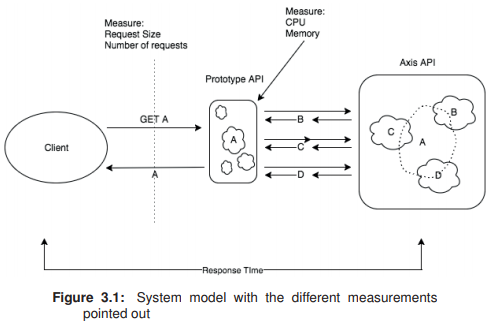
\includegraphics[width=0.8\textwidth]{figuras/metricas.png}
\caption{Arquitetura das APIs e diferentes pontos de medidas}
\label{fig:my-metrics}
\author{fonte: Autor}
\end{figure}

Afim de obter resultados mais precisos, serão feitas diversas iterações para medição de cada umas das métricas. A média destas medições será calculada através da segunte fórmula: 

$$ Avg = \frac{\sum\limits_{1}^{n} X}{n} $$

Onde $n$ é numero de iterações realizadas para cada métrica, e $X$ é o resultado de cada uma destas iterações.

Após a realização dos testes, os dados provenientes de cada uma das métricas foram coletados, analisados e os resultados serão apresentados no próximo capítulo. 
  % ---
  % --- \chapter{Lorem ipsum dolor sit amet}

É importante apresentar, ao início de cada capítulo, uma breve introdução sobre o mesmo. Essa introdução, não deve conter mais do que 2 parágrafos. Uma sugestão, é relembrar de forma sucinta o que foi apresentado no capítulo anterior, e relacionar com o conteúdo deste capítulo.

Também é aconselhável, que cada capítulo possua uma sessão de conclusão. A importância desta é discutida adiante. Esta recomendações não são uma regra do IFC, mas têm sido bastante utilizadas no BSI. 

\section{Figuras e legendas}\label{sec:figs}

Essa sessão apresenta como utilizar figuras e tabelas ao longo do TCC. Também é apresentado o uso das legendas para esses dois tipos de recursos. 

Podemos utilizar tabelas também (tabela~\ref{tab:exTabela}). Nesse caso tente evitar o uso de fundos com cores ou sombras, e evite linhas de grade grossas, duplas ou desnecessárias. A legenda da tabela deve ser colocada sempre antes dela, no topo.

\begin{table}[htbp]
\centering
\caption{Um exemplo de tabela}
\label{tab:exTabela}
\begin{tabular}{l|c|r} \hline
Cabeçalho Esquerda & Cabeçalho Centro & Cabeçalho Direita \\ 
\hline \hline
Linha 1 Coluna 1   & Linha 1 Coluna 2 & Linha 1 Coluna 3  \\
Linha 2            & Coluna do meio   & Coluna 3          \\
Coluna 1           & Linha 3          & Última célula     \\
\hline
\end{tabular}
\end{table}

\section{Códigos-fontes de linguagens de programação}

Uma linguagem de programação é um método padronizado para expressar instruções para um computador. É um conjunto de regras sintáticas e semânticas usadas para definir um programa de computador. Uma linguagem permite que um programador especifique precisamente sobre quais dados um computador vai atuar, como estes dados serão armazenados ou transmitidos e quais ações devem ser tomadas sob várias circunstâncias.

Depois que inventaram o computador , perceberam que ele não servia prá nada. Durante milhares de anos o computador ficou relegado a segundo plano e apenas calculadoras eram usadas! Mas um tecelão francês chamado Jacquard criou o primeiro programa para suas máquinas de tecer. Com inveja, Blaise Pascal, inventou a linguagem Pascal para jovens com retardamento mental. Naquela época os computadores ainda eram muito rudimentares e não foi possível utilizar de forma satisfatória todos os recursos das Linguagens de Programação. Muito tempo depois Charles Babbage criou a máquina Diferencial prá fazer subtrações e a máquina Somatorial para fazer somas. Como dava um trabalho muito duro construir máquinas para cada uma das operações, ele pediu à sua assistente Lady Ada Lovelace prá resolver o problema. Ada então criou a Linguagem de Programação Ada, muito utilizada na Guerra do Golfo pelos Militares Americanos.

\subsection{Python}

Python é uma linguagem de programação de alto-nível interpretada, interativa, orientada a objetos, de tipagem dinâmica e forte. A linguagem foi projetada com a filosofia de enfatizar a importância do esforço do programador sobre o esforço computacional. Prioriza a legibilidade do código sobre a velocidade ou expresividade. Combina uma sintaxe concisa e clara com os recursos poderosos de sua biblioteca padrão e por módulos e frameworks desenvolvidos por terceiros. O código \ref{mediapy} é um exemplo de código-fonte em Python.

Python é a principal sucessora de Logo, porém é também uma calculadora de linha de comando, orientada à identação. Costuma ser o destino preferencial dos programadores Ruby, quando estes finalmente se dão conta que estão usando um ``Perl 2.0''. 

\subsection{C++}

O C++ é uma linguagem de programação de alto nível com facilidades para o uso em baixo nível, multiparadigma e de uso geral. Desde os anos 1990 é uma das linguagens comerciais mais populares, sendo bastante usada também na academia por seu grande desempenho e base de utilizadores.  O código \ref{mediacpp} é um exemplo de código-fonte em C++.


C++ é uma linguagem de programação, muitas vezes é referida como Cpp , criada por Steve Ballmer com o propósito de deixar programador loucos, em um plano para eliminar a concorrência da Microsoft (que usa a programação orientada a gambiarras em seus programas).

Suas principais características são o paradigma orientado à desorientação e falta de sentido em geral, a incoerência de sintaxe, e ser melhor do que Java. A linguagem incorpora todas as vantagens da linguagem C, isto é, nenhuma, e todos os benefícios da orientação a objetos, isto é, poder fazer uma classe Quadrado que herda da classe Retângulo, com um incrivel custo em performance por isso. 

\subsection{Java}

Java é uma linguagem de programação orientada a objeto desenvolvida na década de 90 pelo programador James Gosling, na empresa Sun Microsystems. Diferentemente das linguagens convencionais, que são compiladas para código nativo, a linguagem Java é compilada para um ``bytecode'' que é executado por uma máquina virtual. A linguagem de programação Java é a linguagem convencional da Plataforma Java, mas não sua única linguagem.  O código \ref{mediajava} é um exemplo de código-fonte em Java.


A Linguagem Java é famosa por ser muito eficiente. A maioria dos programas mais complexos é escrita em Java, como o Adobe Photoshop ou o Microsoft Windows ME, podendo funcionar com apenas 640 bytes de RAM, e atingir velocidades instantâneas. Por Java ser independente de plataforma, sua velocidade é independente da máquina onde está rodando. Por padrão, Java 1.2 pode calcular um loop infinito em menos de 1.2 minutos, daí vem esse número na linguagem. A palavra ``Java'' vem de um dialeto da Indonésia que quer dizer ``Espetáculo do crescimento'', o que explica programas com poucos KBytes no disco possuírem dezenas de MBytes na memória principal.

\subsection{Listas numeradas e de itens}

Se quisermos uma lista numerada, devemos fazer assim:

\begin{enumerate}
\item este é o primeiro item;
\item este é o segundo item;
\item e este é o terceiro e último item.
\end{enumerate}

Por outro lado, uma lista de itens é feita desse modo:

\begin{itemize}
\item este é o primeiro item;
\item este é o segundo item;
\item e este é o terceiro e último item.
\end{itemize}

\section{Referências}

Referências bibliográficas precisam ser não ambíguas e uniformes. Recomendamosdar os nomes dos autores entre espaços, por exemplo \cite{knuth:84},
\cite{boulic:91}, e \cite{smith:99}. Em caso de dúvidas, consulte o manual de metodologia para desenvolvimento do TCC, disponível na página do IFC ou na página do BSI.

Citações longas com mais de três linhas devem seguir ao seguinte formato:

\begin{citacao}
O IPSEC foi concebido como uma extensão de terceira camada ao TCP/IP, ou seja estende o próprio protocolo IP. Na verdade, para o IPv6; depois o IPSEC também foi portado para o IPv4.
A idéia original do IPSEC é permitir a comunicação segura e *transparente* entre quaisquer dois nós da Internet, desde que os dois implementem IPSEC. Se os dois têm IPSEC, automaticamente há troca de chaves e criptografia. Esse modo de funcionamento do IPSEC denomina-se ``modo transporte''~\cite{epx}. 
\end{citacao}

% ---
\section{Aliquam vestibulum fringilla lorem}
% ---

\lipsum[1]

\lipsum[2-3]

  % ---
% primeiro capitulo de Resultados
% ---
\chapter{Resultados}

Neste capítulo, os resultados e a análise dos experimentos realizados durante o trabalho são reportados. Os resultados obtidos nos testes de validação apresentam a média dos valores coletados após diversas execuções dos cenários de forma sequencial.

Foram executadas 30 iterações para cada requisição a fim de obter as respostas das questões levantadas no capítulo \ref{cap:estudo}. Os dados necessários puderam ser buscados em uma única requisição à API GraphQL, enquanto foram necessárias duas requisições à API REST para chegar a resposta da primeira questão, e vinte e oito para obter a resposta da segunda. Os detalhes para obter os resultados na API REST podem ser constatados nas tabelas \ref{tab:request-table1} e \ref{tab:request-table2}.

\begin{table}[htbp]
    \centering
    \begin{tabular}{| l | l | l |}
        \hline
        \textbf{Requisição} & \textbf{Resultado} & \textbf{Número de requisições} \\ \hline
        /pallets & Todos os pallets & 1 \\ \hline
        /items/:id & Detalhes do item mais presente & 1 \\ \hline
    \end{tabular}
    \caption{Fluxo de dados para responder Questão 1} 
    \label{tab:request-table1}
\end{table}

\begin{table}[htbp]
    \centering
    \begin{tabular}{| l | l | l |}
        \hline
        \textbf{Requisição} & \textbf{Resultado} & \textbf{Número de requisições} \\ \hline
        /items & ID do item 22B12 & 1 \\ \hline
        /items/:id & Detalhes do item 22B12 & 1 \\ \hline
        /pallets & Pallets contendo item 22B12 & 1 \\ \hline
        /pallets/:id & Detalhes do Pallet contendo o item 22B12 & 5 \\ \hline
        /addresses/:id & Detalhes do Endereço contendo o item 22B12 & 5 \\ \hline
        /levels/:id & Nível contendo o item 22B12 & 5 \\ \hline
        /slots/:id & Prateleira contendo o item 22B12 & 5  \\ \hline
        /rows/:id & Linha contendo o item 22B12 & 5 \\ \hline
    \end{tabular}
    \caption{Fluxo de dados para responder Questão 2} 
    \label{tab:request-table2}
\end{table}

Além das 30 iterações feitas para cada requisição, foram montados também três cenários para melhor análise dos resultados. Estes cenários possuem quantidades de registros diferentes para as entidades \textup{Item} e \textup{Pallet}, pois são estas que afetam de maneira mais significativa o quão eficiente será o desempenho das APIs. Estes três cenários estão descritos na tabela \ref{tab:cenarios} com suas respectivas quantidades.

\begin{table}[htbp]
    \centering
    \begin{tabular}{| l | l | l | l|}
        \hline
        \textbf{Recurso} & \textbf{Cenário 1 (C1)} & \textbf{Cenário 2 (C2)} & \textbf{Cenário 3 (C3)} \\ \hline
        Item & 1000 & 10000 & 30000 \\ \hline
        Pallet & 1000 & 10000 & 30000 \\ \hline
        Address & 156 & 156 & 156 \\ \hline
        Slot & 26 & 26 & 26 \\ \hline
        Row & 2 & 2 & 2 \\ \hline
        Level & 3 & 3 & 3 \\ \hline
    \end{tabular}
    \caption{Cenários analisados} 
    \label{tab:cenarios}
\end{table}

\section{Questão 1}

Embora necessite de buscas mais simples, através da Questão 1 já é possível observar as diferenças em termos de desempenho entre a aplicação REST e a aplicação GraphQL. A Questão 1 busca o item com a maior quantidade de \textit{pallets} alocados no armazém, e para responde-la é necessário duas etapas. A primeira busca todos os \textit{pallets} registrados no sistema, e após identificado qual o item mais comum presente nos \textit{pallets} registrados, a segunda etapa detalha este item, extraindo a descrição dele por exemplo.

\subsection{Tempo de utilização da CPU}

Ao analisar o tempo de utilização da CPU, ilustrada na figura \ref{fig:q1-cpu}, percebe-se que as APIs REST e GraphQL tem desempenho similares nos cenários C1 e C2. Por outro lado, as consultas para o cenário C3, mostram a API REST menos eficiente ao utilizar a CPU.

\begin{figure}[htbp]
    \centering
    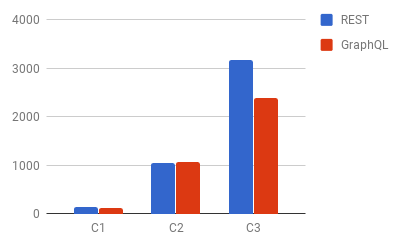
\includegraphics[width=0.8\textwidth]{figuras/q1-cpu.png}
    \caption{Comparação da Utilização de CPU}
    \label{fig:q1-cpu}
\end{figure}

As consultas de C1 exigiram 133,80~ms de CPU na API REST e apenas 111,10~ms na API GraphQL. Executando o cenário C2, a API REST foi processada em 1042,52~ms enquanto a API GraphQL levou 1065,45~ms, e é neste cenário que nota-se a maior similaridade no tempo de utilização da CPU entre as APIs. No entanto, quando analisados os resultados de C3, nota-se uma grande desvantagem para API REST, que utilizou 3177,60~ms da CPU enquanto a API GraphQL usou apenas 2382,10~ms: uma diferença de cerca de 25\%.
    
\subsection{Consumo de memória}

Os dados do resultado da comparação do consumo de memória expõem que a API REST também se mostrou menos eficiente neste quesito em relação à API GraphQL. Os resultados podem ser observados na figura \ref{fig:q1-mem}.

\begin{figure}[htbp]
    \centering
    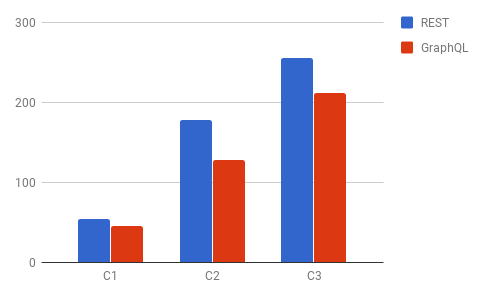
\includegraphics[width=0.8\textwidth]{figuras/q1-memory.png}
    \caption{Comparação do Consumo de Memória}
    \label{fig:q1-mem}
\end{figure}

Ao compararmos os resultados de C1 e C3, a API REST se mostrou cerca de 15\% menos eficiente que a API GraphQL. O que se destaca é quando compara-se os resultados de C2, em que a API GraphQL consumiu 127,71 megabytes de memória e a API REST consumiu 178,01 megabytes, uma diferença de aproximadamente 30\%.

\subsection{Tempo de resposta}

Como esperado, a API implementada com GraphQL realmente respondeu as consultas em um tempo menor do que a API REST. A figura \ref{fig:q1-time} mostra a diferença do tempo de resposta das APIs para executar as consultas da primeira questão.

\begin{figure}[htbp]
    \centering
    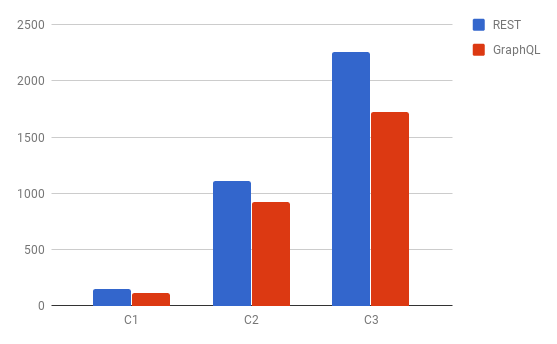
\includegraphics[width=0.8\textwidth]{figuras/q1-time.png}
    \caption{Comparação do tempo de resposta}
    \label{fig:q1-time}
    \author{fonte: Autor}
\end{figure}

Nas requisições de C1, a API REST teve como resultado um tempo de resposta de 147,23~ms, enquanto a API GraphQL respondeu a consulta em 115,63~ms, representando uma diferença de 21\%. Ao analisar as consultas de C2, a API REST respondeu as consultas em 1108,13~ms e a API GraphQL devolveu os resultados em 925,63~ms, uma diferença de 16\%. Por último, as consultas de C3 foram respondidas em 2261,10~ms na API REST e 1725,70~ms na API GraphQL, o que representa uma diferença de 23\%.

Para o tempo de resposta foi extraído mais um gráfico, que pode ser observado na figura \ref{fig:q1-time-line}, que ilustra o tempo de resposta para cada umas das 30 requisições nas duas APIs. Esse gráfico é baseado nas consultas para o cenário C1, e ajuda a explicar o comportamento de tempo de resposta de cada uma das APIs. É possível observar em ambos os protótipos que a primeira requisição leva um tempo bem superior que a média do protótipo. Isso se explica pois na primeira requisição a API precisa de um tempo de \textit{warmup}, necessário para estar em pleno desempenho. Esse período de \textit{warmup} ocorre apenas na primeira requisição e as próximas requisições já se mostram muito mais rápidas.

\begin{figure}[htbp]
    \centering
    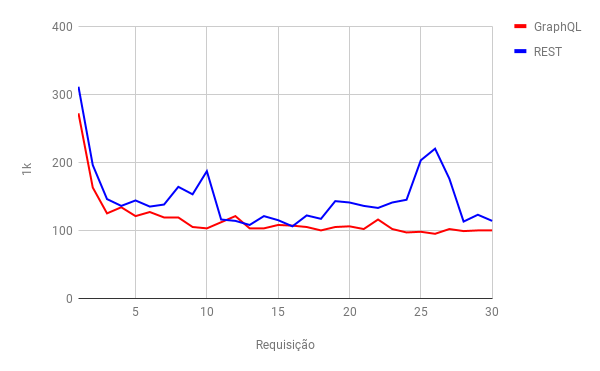
\includegraphics[width=0.8\textwidth]{figuras/q1-time-line.png}
    \caption{Tempo de resposta}
    \label{fig:q1-time-line}
\end{figure}

\subsection{Tamanho da resposta}

Outro resultado esperado era que o tamanho da resposta da API GraphQL fosse menor do que o tamanho da resposta da API REST. Essa hipótese se confirmou como pode ser visto da figura \ref{fig:q1-size}.

\begin{figure}[htbp]
    \centering
    \includegraphics[width=0.8\textwidth]{figuras/q1-size.png}
    \caption{Comparação do tamanho de resposta}
    \label{fig:q1-size}
    \author{fonte: Autor}
\end{figure}

A API REST respondeu as requisições da Questão 1 com um tamanho de resposta de 174,04 kilobytes, 1740,17 kilobytes e 4980 kilobytes para C1, C2, C3 respectivamente. Da mesma maneira, a API GraphQL teve como resultado respostas com 31,68 kilobytes, 322,53 kilobytes e 967,35 kilobytes. Comparando os três cenários é constatado uma diferença constante de cerca de 80\% entre a API REST e a API GraphQL.

%%--------------
%%--------------
%%--------------

\section{Questão 2}

Para as respostas da questão 2, as consultas foram mais complexas na API GraphQL, e mais numerosas na API REST. Estas consultas visaram responder quais são os endereços que contém o Item 22B12, e foi analisando os resultados que é possível identificar a maior diferença de desempenho das APIs, com destaque ao tamanho da resposta obtida.

\subsection{Tempo de utilização da CPU}

Analisando os resultados do tempo utilização de CPU, podemos concluir que a API GraphQL utiliza este recurso de uma maneira mais eficiente do que a API REST. A figura \ref{fig:q2-cpu} ilustra os resultados obtidos.

\begin{figure}[htbp]
    \centering
    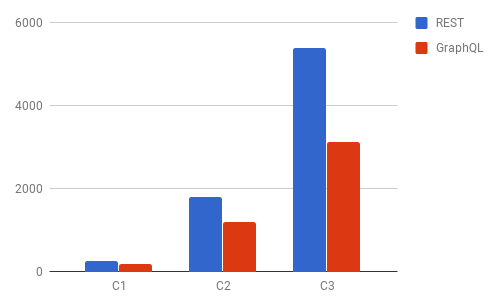
\includegraphics[width=0.8\textwidth]{figuras/q2-cpu.png}
    \caption{Comparação da Utilização da CPU}
    \label{fig:q2-cpu}
    \author{fonte: Autor}
\end{figure}

Aqui a diferença nos resultados obtidos é notada com mais clareza, à medida em que se aumenta o número de registros. Analisando C1, a API REST exigiu 244,41~ms da CPU para ser processada, ao mesmo tempo que a API GraphQL exigiu somente 178,22~ms. Nas consultas de C2, a API REST demandou 1787,74~ms para ser processada, e a API GraphQL demandou 1199,53~ms. A maior diferença encontra-se em C3, onde a API REST levou 5383,40~ms para ser completamente processada pela CPU e a API GraphQL levou apenas 3132,98~ms. No cenário C3 observamos uma diferença de mais de 40\% entre o desempenho das APIs.

\subsection{Consumo de memória}

Os dados referentes ao consumo de memória estão ilustrados na figura \ref{fig:q2-mem}, e apontam que a API REST faz uso menos eficiente deste recurso, comparando com o consumo de memória da API GraphQL. Entretanto, foi analisando esta métrica que se encontrou o único cenário em que a API REST se mostrou mais eficiente que a API GraphQL.

\begin{figure}[htbp]
    \centering
    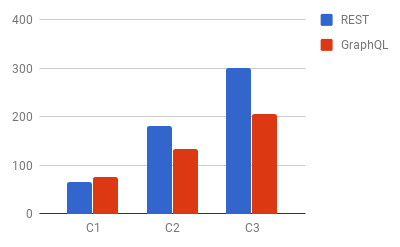
\includegraphics[width=0.8\textwidth]{figuras/q2-memory.png}
    \caption{Comparação do Consumo de memória}
    \label{fig:q2-mem}
    \author{fonte: Autor}
\end{figure}

O consumo de memória não se mostrou tão diferente comparando as APIs nos cenários C1 e C2. Nas requisições de C1, a API REST demonstra ser mais eficiente, mesmo que a diferença seja de apenas 9,88 megabytes (ou 12\%), em relação a API GraphQL. A API GraphQL consumiu 76,19 megabytes de memória, contra 66,27 consumidos pela API REST. Essa melhor eficiência já não é mais identificada em C2, onde a API REST consumiu 181,02 megabytes de memória, e a API GraphQL consumiu 26\% menos, totalizando 133,52 megabytes. Nas consultas de C3, observamos uma diferença relevante no consumo de memória, com a API REST consumindo 300,30 megabytes de memória enquanto a API GraphQL consumiu 206,02 megabytes, uma impressionante diferença de quase 100 megabytes ou 30\%.

\subsection{Tempo de resposta}

Como mostra a figura \ref{fig:q2-time}, é possível identificar com clareza que a API REST leva um tempo consideravelmente maior para responder todas as requisições comparando com o tempo levado pelas consultas na API GraphQL.

\begin{figure}[htbp]
    \centering
    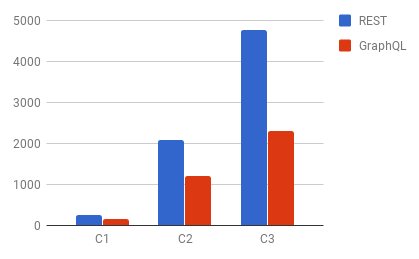
\includegraphics[width=0.8\textwidth]{figuras/q2-time.png}
    \caption{Comparação do tempo de resposta}
    \label{fig:q2-time}
    \author{fonte: Autor}
\end{figure}

Considerando as consultas de C1, a API REST teve como resultado um tempo de resposta de 254,56~ms, enquanto a API GraphQL respondeu a consulta em 148,50~ms, representando uma diferença de pouco mais de 40\%. Quando analisado as requisições de C2, a API REST respondeu as consultas em 2072,03~ms e a API GraphQL devolveu o resultado em 1201,30~ms, uma diferença de 42\%, muito semelhante ao C1. Por último, as consultas de C3 foram respondidas em 4770,20~ms na API REST e 2291,10~ms na API GraphQL, o que representa uma diferença de pouco mais de 50\%.

Como feito na Questão 1, também foi extraído um gráfico ilustrando o tempo de resposta para cada umas das 30 requisições, no cenário C1. Entretanto, diferente do que ocorreu na Questão 1, onde grande parte das requisições levaram tempos muito similares, para a Questão 2 observamos uma diferença muito mais significativa. Os resultados podem ser vistos na figura \ref{fig:q2-time-line}.

\begin{figure}[htbp]
    \centering
    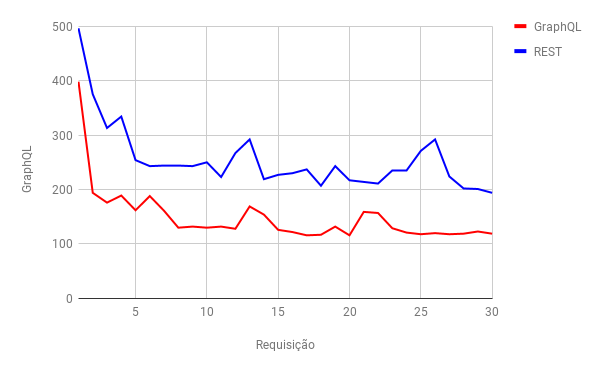
\includegraphics[width=0.8\textwidth]{figuras/q2-time-line.png}
    \caption{Tempo de resposta}
    \label{fig:q2-time-line}
\end{figure}

O período de \textit{warmup} é também facilmente observado na Questão 2. A API REST responde a primeira requisição em quase 500 ms, enquanto a API GraphQL responde a primeira requisição em pouco menos de 400 ms. Essa diferença de quase 100ms se mantém ao decorrer das requisições, sendo que a API GraphQL se mostra um pouco mais estável do que a API GraphQL, sem grandes oscilações.

\subsection{Tamanho da resposta}

A API GraphQL também mostrou-se mais vantajosa em termos de tamanho da resposta na Questão 2. A figura \ref{fig:q2-size} mostra a comparação entre os protótipos levando em consideração o tempo da resposta.

\begin{figure}[htbp]
    \centering
    \includegraphics[width=0.8\textwidth]{figuras/q2-size.png}
    \caption{Comparação do tamanho da resposta}
    \label{fig:q2-size}
    \author{fonte: Autor}
\end{figure}

A API REST respondeu as requisições da questão 1 com um tamanho de resposta de 259,53 kilobytes, 2522.17 kilobytes e 7221,00 kilobytes para C1, C2 e C3 respectivamente. Da mesma maneira, a API GraphQL teve como resultado respostas com 101,73 kilobytes, 1005,23 kilobytes e 2850,00 kilobytes. Como ocorrido da Questão 1, a diferença de desempenho entre as APIs se manteve em torno de 60\% nos três cenários, deixando claro a melhor eficiência da API GraphQL neste quesito.

O GraphQL mostrou-se muito estável nos testes realizados levando em consideração todas as métricas analisadas. Em 7 dos 8 cenários propostos, a API GraphQL apresentou um desempenho superior em relação à API REST.
  
  % ----------------------------------------------------------
  % Finaliza a parte no bookmark do PDF
  % para que se inicie o bookmark na raiz
  % e adiciona espaço de parte no Sumário
  % ----------------------------------------------------------
  \phantompart
  
  % ---
% Conclusão
% ---
\chapter{Conclusão}
% ---

Com cada vez mais dispositivos interconectados, a eficiência na comunicação entre aplicações é um tema que está em constante debate e evolução. Recursos computacionais como memórias e processadores, embora gradativamente mais acessíveis, ainda demandam preocupação em relação ao seu uso sustentável, principalmente levando em consideração serviços \textit{on demand} em nuvem.

Este trabalho apresentou conceitos e modelos de comunicação entre aplicações, abrangendo algumas de suas vantagens e desvantagens. Além disso, foram levantadas quatro hipóteses referentes ao desempenho de APIs implementando protótipos de dois dos modelos apresentados: REST e GraphQL. Com a utilização dos modelos, um experimento foi realizado para compará-los. A realização do experimento mensurou o desempenho das APIs em termos de tempo de resposta, quantidade de banda utilizada e consumo de recursos computacionais.

A primeira hipótese sugeria que o tamanho da resposta seria menor para as consultas à API GraphQL. Os resultados do experimento consolidaram esta hipótese como verdadeira, mostrando que a API GraphQL foi em todos os cenários propostos mais eficiente do que a API REST, sendo que em alguns cenários a diferença entre as duas APIs foi de quase 80\%. Este resultado já era esperado, pois como princípio, APIs REST expõem recursos, e a consulta destes recursos sempre retornam a representação completa dos objetos. Ainda, APIs GraphQL respondem apenas os campos solicitados pela consulta, resultando em respostas mais concisas.

A segunda hipótese declarava que o tempo de resposta também seria menor para as consultas à API GraphQL. Novamente os resultados confirmaram esta hipótese, e em nenhum dos cenários a API REST se mostrou mais eficiente do que a API GraphQL neste quesito. Em um dos cenários, a API GraphQL respondeu a consulta na metade do tempo necessário para a API REST, sendo que em nenhum cenário a diferença foi menor do que 15\%. Os resultados da primeira hipótese podem ajudar um pouco a explicar por que os tempos de resposta da API GraphQL são menores do que os tempos da API REST. Uma vez que é preciso trafegar menos informações pela rede, as consultas são naturalmente respondidas mais rapidamente. Também, outro fator que influencia o tempo de resposta, é quanto tempo a consulta leva para ser processada.

A terceira hipótese afirmava que o tempo de utilização da CPU para as requisições REST seria maior do que o tempo para as requisições GraphQL. Os resultados mostraram que embora em um dos cenários a utilização da CPU foi praticamente igual entre as duas APIs, a medida que é necessário realizar consultas em objetos maiores, o tempo de utilização da CPU da API REST aumenta signitivamente, alcançando uma diferença de mais de 40\% em relação a API GraphQL.

A última hipótese alegava que o consumo de memória da API REST seria menor do que o consumo de memória da API GraphQL. Outra vez, os resultados refutaram esta hipótese. Foi ao avaliar este quesito que o único cenário em que a API REST teve uma eficiência maior do que a API GraphQL foi encontrado. Entretanto, enquanto a diferença de desempenho entre as API foi de apenas 12\% no cenário favorável ao REST, no cenário em que o GraphQL foi mais eficiente, a diferença foi de 30\%. 

Ao fim do trabalho conclui-se que ambas as tecnologias oferecem uma solução prática e eficiente para o mesmo problema, entretanto o GraphQL apresenta-se como uma ótima alternativa como mecanismo de comunicação entre aplicações. A facilidade de uso, menor consumo de recursos computacionais e de banda contribuem para que o GraphQL seja uma ferramenta muito utilizada futuramente pelas organizações e desenvolvedores. 

Por outro lado, os critérios de desempenho podem não ser os únicos benefícios trazidos com a utilização do GraphQL. Posto que, os desenvolvedores das aplicações clientes são encarregados de definir cada requisição, eles podem ser bastante seletivos em relação os dados trafegados. Desde modo, o GraphQL ajuda a maximizar a produtividade do desenvolvimento de aplicações, resultando em uma melhor \textit{Developer Experience} (DX), uma disciplina que vem ganhando cada vez mais dedicação e importância dentro das empresas.

Contudo, a maturidade o ecosistema GraphQL ainda é uma questão muito discutida pela comunidade. Embora ele tenha sido usado internamente pelo Facebook por anos, o GraphQL só foi apresentado a um público mais amplo em 2015, e foi apenas em 2016 que o Facebook transferiu seu \textit{status} para \textit{production-ready}.

Trabalhos futuros poderiam abordar como a utilização de arquiteturas baseadas em JSON/Graphs (GraphQL, Falcor), podem otimizar o desenvolvimento de \textit{softwares}, não apenas em uma maneira quantitativa, mas também de maneiras qualitativas, levando em consideração a \textit{Developer Experience}. Outros trabalhos também poderiam abordar as vantagens de ter uma comunicação fortemente tipada, como ocorre com o GraphQL. Ou ainda, se a teoria das categorias pode ser aplicada através do GraphQL.

  
  % ----------------------------------------------------------
  % ELEMENTOS PÓS-TEXTUAIS
  % ----------------------------------------------------------
  \postextual
  % ----------------------------------------------------------
  
  % ----------------------------------------------------------
  % Referências bibliográficas
  % ----------------------------------------------------------
  \bibliography{referencias}
  
  % ----------------------------------------------------------
  % Glossário
  % ----------------------------------------------------------
  %
  % Consulte o manual da classe abntex2 para orientações sobre o glossário.
  %
  %\glossary
  
  % ----------------------------------------------------------
  % Apêndices
  % ----------------------------------------------------------
  
  % ---
  % Inicia os apêndices
  % ---
  \begin{apendicesenv}
  
  
  \end{apendicesenv}
  % ---
  
  
  % ----------------------------------------------------------
  % Anexos
  % ----------------------------------------------------------
  
  % ---
  % Inicia os anexos
  % ---
  \begin{anexosenv}
  
  
  \end{anexosenv}
  
  %---------------------------------------------------------------------
  % INDICE REMISSIVO
  %---------------------------------------------------------------------
  \phantompart
  \printindex
  %---------------------------------------------------------------------
  
  \end{document}
  